\chapter{Анализ прикладных задач выбора моделей машинного обучения}
Планирование эксперимента требует оценки минимального размера выборки: числа выполненных измерений набора характеристик, необходимых для построения сформулированных условий. Выбор метода оценки размера выборки зависит от решаемой задачи, которая определяет формулировку статистической гипотезы и статистики для ее проверки. В таблице \ref{table1} представлены десять методов оценки размера выборки. Они включают как статистические, так и байесовский методы оценки размера выборки.

Статистические методы предполагают, что выборка соответствует некоторым предварительным условиям, сформулированным ранее. Эти условия сформулированы как статистический критерий~\cite{self1988,self1992,shieh2000,demidenko2007}. Метод оценки размера выборки, связанный с этим критерием, гарантирует достижение фиксированной статистической мощности~$1-\beta$ со степенью ошибки первого рода, не превышающей установленное значение~$\alpha$. Такой размер выборки называется достаточным.

\begin{table}
\begin{center}
\caption{Сводная таблица методов определения оптимального размера выборка для линейных моделей}
\label{table1}
\resizebox{\textwidth}{!}{
\begin{tabular}{|p{0.15\textwidth}|p{0.6\textwidth}|p{0.15\textwidth}|}
\hline
	\centering Метод &\centering Описание & Ссылка\\
\hline
	Lagrange multipliers test &
	Правдоподобие выборки имеет вид:
   	$p(y|\textbf{x}, \textbf{w}) = \exp\bigl(y\theta- b(\theta) + c\left(y\right)\bigr).$
	Достаточный размер выборки~$m^*$:
	$m^* = \frac{\gamma^*}{\gamma^0}$, где~$\gamma^*$ и~$\gamma_0$ задаются выражениям \eqref{eq:sb:6} и \eqref{eq:sb:5}.
	&\cite{self1988}\\
\hline
	Likelihood ratio test&
	Правдоподобие выборки имеет вид:
	$p(y|\textbf{x}, \textbf{w}) = \exp\left(\frac{y\theta- b(\theta)}{a(\phi)} + c\left(y, \phi\right)\right).$
	Достаточный размер выборки~$m^*$:
	$m^* = \frac{\gamma^*}{\Delta^*},$ где~$\gamma^*$ и~$\Delta^*$ задаются вывражениями \eqref{eq:sb:11} и \eqref{eq:sb:13}.
	&\cite{shieh2000}\\
\hline
	Wald statistic&
	Правдоподобие выборки имеет вид:
	$p(y|\textbf{x}, \textbf{w}) = \exp\left(\frac{y\theta- b(\theta)}{a(\phi)} + c\left(y, \phi\right)\right).$
	
	Достаточный размер выборки~$m^*$:
	
	$m^* = \frac{\gamma^*}{\delta},$ где~$\gamma^*$ и~$\delta$ задаются выражением \eqref{eq:sb:20}.
	&\cite{shieh2005}\\
\hline
	Cross-validation&
	
	Достаточный размер выборки~$m^*$:
	
	$ \forall m \geq m^* RS(m) \geq 1- \varepsilon,$
	где~$\varepsilon$ задается экспертно,~$RS$ определяется выражением \eqref{eq:hb:5}.
	&\cite{motrenko2014}\\
\hline
	Bootstrap&
	
	Достаточный размер выборки~$m^*: \forall m\geq m^* \max_i\left(b^m_i - a^m_i\right) < l$, где~$(a^m_i,  b^m_i)$ является квантилью доверительного интервала~$i$-й бутсрап подвыборки размера~$m$

	&\cite{qumsiyeh2013}\\
\hline
	Kullback-Leibler&
	
	Достаточный размер выборки~$m^*$:
	
	$\forall \mathfrak{D}_{\mathcal{B}_1}: \left|\mathfrak{D}_{\mathcal{B}_1}\right| \geq m^*    \mathsf{E}_{\mathfrak{D}_{\mathcal{B}_2}}D_\text{KL}\left(p_1, p_2\right) \leq \varepsilon,$
	где~$\mathcal{B}_1, \mathcal{B}_2$ удовлетворяет \eqref{eq:bs:8}.
	&\cite{motrenko2014}\\
\hline
	Average posterior variance criterion&
	
	Достаточный размер выборки~$m^*$:
	
	$\forall m \geq m^*    \mathsf{E}_{\mathfrak{D}_m}\mathsf{D}\left[\hat{\textbf{w}}|\mathfrak{D}_m\right] \leq \varepsilon,$ где~$\varepsilon$  достаточно малое значение.
	&\cite{joseph1995,joseph1997}\\
\hline
	Average coverage criterion&
	Достаточный размер выборки~$m^*$:
	
	$\forall m \geq m^*    \mathsf{E}_{\mathfrak{D}_m}\mathsf{P}\left\{\textbf{w} \in A\left(\mathfrak{D}_m\right)\right\} \geq 1-\alpha$, где~$\alpha$ достаточно малое значение.
	&\cite{joseph1995,joseph1997}\\
\hline
	Average length criterion&
	Достаточный размер выборки~$m^*$:
	
	$\forall m \geq m^*    \mathsf{E}_{\mathfrak{D}_m}r_m\leq l,$ 
	where~$r_m$ is described in \eqref{eq:bs:5}
	&\cite{joseph1995,joseph1997}\\
\hline
	Utility maximization&
	Достаточный размер выборки~$m^*$:
	
	$m^* = \arg\max_{m} \mathsf{E}_{\mathfrak{D}_m}\int_{\textbf{w}}u\left(\mathfrak{D}, \textbf{w}\right)p(\textbf{w}|\mathfrak{D})d\textbf{w},$
	где функция полезности~$u\left(\mathfrak{D}, \textbf{w}\right)$ задается выражением \eqref{eq:bs:7}.
	&\cite{lindley1997}\\


\hline
\end{tabular}
}
\end{center}
\end{table}

Однако практическое применение методов оценки размера выборки предполагает, что модель соответствует измеренным данным~\cite{kloek1975}. Эти модели выбираются в соответствии с постановкой задачи регрессии или классификации. В этой статье представлены обобщенные линейные модели. В статье~\cite{self1992} предложен подход к оценке мощности и размера выборки, связанной с ней, на основе теста отношения максимального правдоподобия. Этот подход оказался более точным для ряда независимых переменных. Кроме того, в статье~\cite{shieh2005} предложен метод оценки мощности для статистики Вальда. В статье~\cite{motrenko2014} в случае логистической регрессии предлагается использовать метод, использующий кривую ROC-AUC и концепцию сдвига. Классические методы~\cite{self1988,self1992,shieh2000,shieh2005,demidenko2007} имеют ряд ограничений, связанных с практическим применением этих методов. Чтобы оценить размер выборки, необходимо знать дисперсию оценки параметра или, в более общем случае, иметь оценку параметра нецентральности в распределении статистики, используемой, когда альтернативная гипотеза верна. Эти методы не показывают как получить эти значения. Кроме того, дисперсия оценки и параметр нецентральности не будут получены с определенной дисперсией, влияние которой на результат оценки размера выборки не имеет значения.

Статистические методы позволяют оценить размер выборки на основе предположений о распределении данных и информации о соответствии между наблюдаемыми значениями и предположениями нулевой гипотезы. Когда размер исследуемой выборки является достаточным или чрезмерным, можно использовать методы, основанные на наблюдении изменения определенной характеристики процедуры построения модели при увеличении размера выборки. В частности, наблюдая за соотношением качества прогнозирования с контрольной выборкой и обучающей выборкой~\cite{motrenko2014}, определяется достаточный размер выборки, который соответствует началу переобучения. В статье~\cite{qumsiyeh2013} для оценки достаточного размера выборки используется процедуру бутстрап. Превышение текущего размера выборки проверяется на основе анализа доверительных интервалов оцениваемого параметра. Ширина доверительного интервала с разными значениями объема выборки оценивается с помощью метода бутстрапа. Для этого выборки меньшего размера отбираются заданное число раз и вычисляется доверительный интервал ошибки при оценке параметра модели. Размер выборки считается достаточным, если ширина доверительного интервала не превышает заранее установленного значения.

Перечисленные выше ограничения статистических методов оценки размера выборки подробно исследуются в байесовской процедуре~\cite{lindley1997,rubin1998,wang2002}, где оценка размера выборки определяется на основе максимизации ожидаемого значение некоторой функции качества~\cite{lindley1997}. Функция качества может включать в себя явные функции распределения параметров и штрафы за увеличение размера выборки. Альтернативой подходам~\cite{wang2002}, основанным на функции качества, является выборка размера выборки путем установления ограничений на определенный критерий качества оценки параметров модели. Примеры критериев: критерий средней апостериорной дисперсии (AVPC), критерий средней длины (ALC), критерий среднего покрытия (ACC). Для каждого перечисленного критерия оценка размера выборки определяется как минимальное значение размера выборки, для которого ожидаемое значение выбранного критерия не превышает какого-либо фиксированного порога. В статье~\cite{motrenko2014} предлагается считать размер выборки достаточным, если расстояние Кульбака-Лейблера между распределениями, оцененными на основе подвыборок такого размера, достаточно мало. Такой подход не требует дальнейшего обобщения в случае нескольких переменных. Кроме того, оценка может производиться как при наличии предположений о распределении данных, так и при их отсутствии. Недостаток этого подхода заключается в том, что количественная оценка может быть получена только при чрезмерно большом размере выборки.

\section{Постановка задачи определения достаточного размера выборки}

Задана выборка размера~$m$:
\[
\label{eq:ps:1}
\begin{aligned}
	\mathfrak{D}_{m} = \{\textbf{x}_i, y_i\}_{i = 1}^{m},
\end{aligned}
\]
где~$\textbf{x}_i\in \mathbb{R}^{n}$,~$y_i\in \mathbb{Y}$. Вектор признаков~$\textbf{x} = [\textbf{u}, \textbf{v}]$ соединяет~$\textbf{u}_i\in \mathbb{R}^{k}$ and~$ \textbf{v}_i\in \mathbb{R}^{n-k}$.
Выборка~$\mathfrak{D}_{m}$ случайным образом делиться на обучающую и тестовую части:
\[
\label{eq:ps:2}
\begin{aligned}
	\mathfrak{D}_{\mathcal{T}_{m}} = \{\textbf{x}_i, \textbf{y}_i\}_{i \in \mathcal{T}_{m}}, \quad \mathfrak{D}_{\mathcal{L}_{m}} = \{\textbf{x}_i, \textbf{y}_i\}_{i \in \mathcal{L}_{m}}, \quad  \mathcal{T}_{m}\sqcup\mathcal{L}_{m} = \{1, ..., m\}.
\end{aligned}
\]
Введем параметрическое семейство функций для аппроксимации неизвестного распределения~$p(y|\textbf{x}, \mathfrak{D}_{\mathcal{L}_{m}})$:
\[
\label{eq:ps:3}
\begin{aligned}
	\mathfrak{F} = \left\{f\left(y,\textbf{x}, \textbf{w}\right)|\textbf{w}\in\mathbb{W}, \int_{y\in \mathbb{Y}, \textbf{x}\in\mathbb{R}^{n}}f\left(y, \textbf{x}, \textbf{w}\right)dyd\textbf{x}=1\right\}.
\end{aligned}
\]

Для модели~$f$ с вектором параметров~$\textbf{w}$ определим функцию правдоподобия и логарифм функции прадоподобия выборки~$\mathfrak{D}$:
\[
\label{eq:ps:4}
\begin{aligned}
	L\left(\mathfrak{D}, \textbf{w}\right) = \prod f\left(y,\textbf{x}, \textbf{w}\right),\quad l\left(\mathfrak{D}, \textbf{w}\right) = \sum \log f\left(y,\textbf{x}, \textbf{w}\right),
\end{aligned}
\]
где~$f(y,\textbf{x}, \textbf{w})$ является оценкой правдоподобия выборки~$\mathfrak{D}_{\mathcal{L}}$ с заданым вектором параметров~$\textbf{w}$.
Используя принцип максимального правдоподобия для оценки параметров~$\textbf{w}$
\[
\label{eq:ps:5}
\begin{aligned}
	\hat{\textbf{w}} = \arg\max_{\textbf{w}\in\mathbb{W}}L\left(\mathfrak{D}_{\mathcal{L}}, \textbf{w}\right).
\end{aligned}
\]

Информационная матрица Фишера имеет вид:
\[
\label{eq:ps:6}
\begin{aligned}
	\textbf{I}\left(\mathfrak{D}, \textbf{w}\right) = -\nabla\nabla^{\mathsf{T}}l\left(\mathfrak{D}, \textbf{w}\right), \quad  \textbf{V} = \textbf{I}^{-1}\left(\mathfrak{D}, \textbf{m}\right),
\end{aligned}
\]
статистические методы и байесовские методы используют информационную матрицу Фишера для оценки размера выборки.

\section{Байесовский подход к определению достаточного размера выборки}

\paragraph{Статистические методы определения достаточного размера выборки.}
Основным преимуществом методов, основанных на статистике, является их способность оценивать достаточный размер выборки при недостаточном наборе выборки. Они позволяют прогнозировать необходимое число образцов на ранней стадии эксперимента.

Плотность распределения целевой переменной
\[
\label{eq:sb:1}
\begin{aligned}
	p(y|\textbf{u},\textbf{v},\textbf{w}_{u},\textbf{w}_{v}) = \exp\bigl(y\theta- b(\theta) + c\left(y\right)\bigr),
\end{aligned}
\]
где~$\theta$ является параметром распределения, полученный с помощью функции связи~$\theta=\theta\bigr(\textbf{u},\textbf{v},\textbf{w}_{u},\textbf{w}_{v}\bigr)$.

Тестируемая гипотеза
\[
\label{eq:sb:2}
\begin{aligned}
	H_0: \textbf{m}_{u} = \textbf{m}^0_{u}, \quad H_1: \textbf{m}_{u} \not= \textbf{m}^0_{u}.
\end{aligned}
\]

Пусть статистики~$S_{m,u}\left(\textbf{w}_{u}, \textbf{w}_{v}\right)$ и~$S_{m,v}\left(\textbf{w}_{u}, \textbf{w}_{v}\right)$ являются производными логарифма правдоподобия выборки~$\mathfrak{D}_{m}$ в точках~$\textbf{w}_{u}$ и~$\textbf{w}_{v}$.
Рассмотрим~$\textbf{s}_{m} = S_{m,u}\left(\textbf{m}^{0}_{u}, \hat{\textbf{w}}^{0}_{v}\right)$, где~$\hat{\textbf{w}}^{0}_{v}$ получается из уравнения
\[
\label{eq:sb:3}
\begin{aligned}
	S_{m,v}\left(\textbf{m}^{0}_{u}, \textbf{w}_{v}\right) = 0.
\end{aligned}
\]
Статистика Лагранджа равняется
\[
\label{eq:sb:4}
\begin{aligned}
	LM = \textbf{s}^{\mathsf{T}}_{m}\textbf{Q}_{m}^{-1}\textbf{s}_{m}.
\end{aligned}
\]
где~$\textbf{Q}_{m}$ ковариационная матрица вектора~$\textbf{s}_{m}$.
	
В случае истинности гипотезы~$H_0$ статистика~$LM$ асимптотически имеет распределения~$\chi^2(k)$.  В~\cite{self1988} показано, что при альтернативной гипотезе~$H_1$ статистика ~$LM$ асимптотически имеет распределения~$\chi^2(k,\gamma)$, где~$\gamma$ является параметром нецентральности
\[
\label{eq:sb:5}
\begin{aligned}
	\gamma = \bm{\xi}_{m}^{\mathsf{T}}\bm{\Sigma}^{-1}_{m}\bm{\xi}_{m} = m\bm{\xi}^{\mathsf{T}}\bm{\Sigma}^{-1}\bm{\xi}= m\gamma^0,
\end{aligned}
\]
где~$\bm{\xi}_{m}$ и~$\bm{\Sigma}_{m}$ матрицы математического ожидания и ковариации~$\textbf{s}_{m}$. Обозначим~$\bm{\xi}_1 = \bm{\xi}$, ~$\bm{\Sigma}_1 = \bm{\Sigma}$. 
	
Альтернативный метод получения~$\gamma$ включает условия на уровне значимости~$\alpha$ и вероятность ошибки II рода~$\beta$:
\[
\label{eq:sb:6}
\begin{aligned}
	\gamma^*:\chi^2_{k, 1-\alpha} = \chi^2_{k, \beta}\left(\gamma\right).
\end{aligned}
\]
Используя \eqref{eq:sb:5} и \eqref{eq:sb:6} получаем
\[
\label{eq:sb:7}
\begin{aligned}
	m^* = \frac{\gamma^*}{\gamma^0}.
\end{aligned}
\]
Это достаточный минимальный размер выборки, чтобы различить вектор~$\textbf{m}_{u}$ от~$\textbf{m}^0_{u}$.

Пусть правдоподобие выборки задается выражением
\[
\label{eq:sb:8}
\begin{aligned}
	p(y|\textbf{u},\textbf{v},\textbf{w}_{u},\textbf{w}_{v}) = \exp\left(\frac{y\theta- b(\theta)}{a(\phi)} + c\left(y, \phi\right)\right),
\end{aligned}
\]
где~$\theta$ является параметром распределения, который вычисляются с помощью функции связи~$\theta=\theta\bigr(\textbf{u},\textbf{v},\textbf{w}_{u},\textbf{w}_{v}\bigr)$.

Проверяемая гипотеза
\[
\label{eq:sb:9}
\begin{aligned}
	H_0: \textbf{m}_{u} = \textbf{m}^0_{u}, \quad H_1: \textbf{m}_{u} \not= \textbf{m}^0_{u}.
\end{aligned}
\]
Введем логарифм статистики отношения правдоподобий:
\[
\label{eq:sb:10}
\begin{aligned}
	LR = 2\Big(l\left(\mathfrak{D}, \hat{\textbf{w}}\right) - l\left(\mathfrak{D}, \hat{\textbf{w}}^0\right)\Big),
\end{aligned}
\]
где~$\hat{\textbf{w}} = [\hat{\textbf{w}}_{u},\hat{\textbf{w}}_{v}]$ является вектором, который максимизирует правдоподобие \eqref{eq:sb:8},~$\hat{\textbf{w}}^{0} = [\textbf{m}^{0}_{u},\hat{\textbf{w}}^{0}_{v}]$ является вектором, который максимизирует правдоподобие \eqref{eq:sb:8} с фиксируемым подвектором параметров~$\textbf{m}^{0}_{u}$.

В случае истинности гипотезы~$H_0$ статистика~$LR$ асимптотически имеет распределения~$\chi^2(k)$.  В~\cite{shieh2000} показано, что при альтернативной гипотезе~$H_1$ статистика ~$LR$ асимптотически имеет распределения~$\chi^2(k,\gamma)$, где~$\gamma$ является параметром нецентральности
\[
\label{eq:sb:11}
\begin{aligned}
	\gamma = m\Delta^*, \quad \Delta^* = \mathsf{E}\left[2a^{-1}(\phi)\left\{\left(\theta - \theta^*\right)\nabla b(\theta) - b(\theta) + b(\theta^*)\right\}\right], 
\end{aligned}
\]
где параметры~$\theta$ и~$\theta^*$ рассчитываются с использованием параметров~$\textbf{w} = [\textbf{w}_{u}, \textbf{w}_{v}]$ и~$\textbf{w}^* = [\textbf{w}^{0}_{u}, \textbf{w}^{*}_{v}]$. Параметры~$\textbf{w}^{*}_{v}$ вычисляются на основе решения уравнения
\[
\label{eq:sb:12}
\begin{aligned}
	\lim_{m\to\infty}m^{-1}\mathsf{E}\left(\frac{\partial l\left(\mathfrak{D}, \left[\textbf{m}^{0}_{u}, \textbf{w}_{v}\right]\right)}{\partial \textbf{w}_{v}}\right) = 0.
\end{aligned}
\]
	
Тогда с учетом~$\alpha$ и~$\beta$ достаточный размер выборки~$m^*$ вычисляется
\[
\label{eq:sb:13}
\begin{aligned}
	m^* = \frac{\gamma^*}{\Delta^*}, \quad \gamma^*:\chi^2_{k, 1-\alpha} = \chi^2_{k, \beta}\left(\gamma\right), 
\end{aligned}
\]
где~$\chi^2_{k, 1-\alpha}$,~$\chi^2_{k, \beta}\left(\gamma^*\right)$ квантили распределений~$\chi^{2}_k$ and~$\chi^2_{k}\left(\gamma^*\right)$.
Правдоподобие выборки:
\[
\label{eq:sb:14}
\begin{aligned}
	p(y|\textbf{u},\textbf{v},\textbf{w}_{u},\textbf{w}_{v}) = \exp\left(\frac{y\theta- b(\theta)}{a(\phi)} + c\left(y, \phi\right)\right),
\end{aligned}
\]
где~$\theta$ является параметром распределения, который вычисляются с помощью функции связи~$\theta=\theta\bigr(\textbf{u},\textbf{v},\textbf{w}_{u},\textbf{w}_{v}\bigr)$.

Тестируемая гипотеза:
\[
\label{eq:sb:15}
\begin{aligned}
	H_0: \textbf{m}_{u} = \textbf{m}_{u}^{0}, \quad H_1: \textbf{m}_{u} \not=\textbf{m}_{u}^{0}.
\end{aligned}
\]
Тест Вальда для гипотезы:
\[
\label{eq:sb:16}
\begin{aligned}
	W = \left(\hat{\textbf{w}}_{u} - \textbf{m}_{u}^{0}\right)^{\mathsf{T}}\hat{\textbf{V}}_{u}^{-1}\left(\hat{\textbf{w}}_{u} - \textbf{m}_{u}^{0}\right),
\end{aligned}
\]
где~$\hat{\textbf{w}} = [\hat{\textbf{w}}_{u},\hat{\textbf{w}}_{v}]$ вектор параметров, который максимизирует правдоподобие выборки \eqref{eq:sb:14}, где матрица~$\hat{\textbf{V}}_u$ задается в выражении \eqref{eq:ps:6}.

В случае истинности гипотезы~$H_0$ статистика Вальда~$W$ асимптотически имеет распределение~$\chi^2$. В~\cite{shieh2005} показано, что в случае истинности альтернативной гипотезы~$H_1$ статистика Вальда~$W$ асимптотически имеет распределение~$\chi^2(k,\gamma)$ с параметром нецентральности~$\gamma$:
\[
\label{eq:sb:17}
\begin{aligned}
	\gamma = m\delta, \quad \delta = \left(\hat{\textbf{w}}_{u} - \textbf{m}_{u}^{0}\right)^{\mathsf{T}}\bm{\Sigma}^{-1}_u\left(\hat{\textbf{w}}_{u} - \textbf{m}_{u}^{0}\right), \quad \bm{\Sigma}_u = m\hat{\textbf{V}}_u.
\end{aligned}
\]

Использую заданный уровень значимости~$\alpha$ и заданную ошибку второго рода~$\beta$ определим оптимальный размер выборки:
\[
\label{eq:sb:18}
\begin{aligned}
	m^* = \frac{\gamma^*}{\delta}, \quad \gamma^*:\chi^2_{k, 1-\alpha^{*}} = \chi^2_{k, \beta}\left(\gamma\right),
\end{aligned}
\]
где~$\chi^2_{k, 1-\alpha^*}$,~$\chi^2_{k, \beta}\left(\gamma^*\right)$ квантили распределения, а параметр~$\alpha^*$ это поправка на уровень значимости:
\[
\label{eq:sb:19}
\begin{aligned}
	\alpha^* = P\left(\bm{\xi}^{\mathsf{T}}\bm{\Sigma}^{*-1} \bm{\xi} > \chi^2_{k,1 - \alpha}\right), \quad \Sigma^* = \textbf{I}^{-1}\left(\mathfrak{D}, \textbf{w}^*\right),
\end{aligned}
\]
где~$\textbf{w}^{*} = \left[\textbf{m}_{u}^{0}, \textbf{w}^{*}_v\right]$ является решением уравнения
\[
\label{eq:sb:20}
\begin{aligned}
	\lim_{m\to\infty}m^{-1}\mathsf{E}\left(\frac{\partial l\left(\mathfrak{D}, \left[ \textbf{m}_{u}^{0}, \textbf{w}_{v}\right]\right)}{\partial \textbf{w}_{v}}\right) = 0.
\end{aligned}
\]

\paragraph{Эвристические методы определения достаточного размера.}
В методе, основанном на эвристике, используются популярные статистические эвристики, такие как бутстрап, перекрестная проверка и задание функции полезности.
Введем набор индексов~$\mathcal {A}~$ для параметров логистической регрессии~$\textbf {w}~$. Тестируется гипотеза
\[
\label{eq:hb:1}
\begin{aligned}
	H_0: j \not\in\mathcal{A} \left(\text{w}_{j} = 0\right), \quad H_1: j \in \mathcal{A}^* \left(\text{w}_{j} \not= 0\right),
\end{aligned}
\]
где~$\text{w}_{j}$ является~$j$-м элементом вектора~$\textbf{w}$.
Установим параметр отступа~$ c_0~$ для задачи логистической регрессии:
\[
\label{eq:hb:2}
\begin{aligned}
	H_0: 1-c_0 = p_0, \quad H_1: 1-c_0 = p_1,
\end{aligned}
\]
где~$c_0$ оптимальное решение, когда исключен~$j$-й элемент вектора.
Используя статистику
\[
\label{eq:hb:3}
\begin{aligned}
	Z = \frac{\hat{p}-p_0}{\sqrt{p_0(1-p_0)}}\sqrt{m}, \quad \hat{p} = \frac{1}{m}\sum_{i=1}^{m}y_i.
\end{aligned}
\]
В случае истинности нулевой гипотезы~$H_0$ статистика~$Z$ асимптотически имеет распределение~$\mathcal{N}\left(0, 1\right)$. В случае истинности альтернативной гипотезы~$H_1$ статистика~$Z$  асимптотически имеет распределение~$ \mathcal{N}\left(p_1-p_0, \sqrt{\frac{p_1(1-p_1)}{p_0(1-p_0)}}\right)$.
      
Достаточный объем выборки задается выражением
\[
\label{eq:hb:4}
\begin{aligned}
	m^* = \frac{p_0(1-p_0)\left(Z_{1-\alpha/2} + Z_{1-\beta}\sqrt{\frac{p_1(1-p_1)}{p_0(1-p_0)}}\right)^2}{(p_1-p_0)^2},
\end{aligned}
\]
где~$Z_{1-\alpha/2}$ и~$Z_{1-\beta}$ являются квантилями распределения~$\mathcal{N}\left(0, 1\right)$.
    
Данный метод не рассматривается далее, поскольку его можно использовать только в задаче логистической регрессии.

Рассмотрим метод на основе кроссвалидации. Определим критерий переобучения как
\[
\label{eq:hb:5}
\begin{aligned}
	RS(m) = \ln\frac{L(\mathfrak{D}_{\mathcal{L}(m)}, \hat{\textbf{w}})}{L(\mathfrak{D}_{\mathcal{T}(m)}, \hat{\textbf{w}})}, \quad \frac{|\mathcal{T}(m)|}{|\mathcal{L}(m)|} = \text{const} \leq 0.5.
\end{aligned}
\]
Заметим, что
\[
\label{eq:hb:6}
\begin{aligned}
	\lim_{m\to \infty}RS(m) \to 0.
\end{aligned}
\]

Достаточный размер выборки~$m^*$ определяется согласно условию:
\[
\label{eq:hb:7}
\begin{aligned}
	m^*: \forall m \geq m^* \mathsf{E}_{\mathfrak{D}_{m}}RS(m) \leq \varepsilon,
\end{aligned}
\]
где~$\varepsilon$ некоторый параметр, который задается экспертно.

Этот метод предполагает, что длины доверительных интервалов квантиля не превышают некоторого фиксированного значения~$l$. Для некоторого размера выборки~$m$ вычисляются квантильные доверительные интервалы~$\left (a^m_1, b^m_1\right), \left(a^m_2, b^m_2 \right), ..., \left(a^m_n, b^m_n \right)$ с уровнем значимости~$\alpha$ с использованием начальной загрузки для каждого параметра модели. Достаточный размер выборки задается выражением:
\[
\label{eq:hb:8}
\begin{aligned}
	m^*: \forall m\geq m^* \max_i\left(b^m_i - a^m_i\right) < l.
\end{aligned}
\]
    
Важно, что этот метод является покоординатным и следовательно для повышения точности прогноза требуется значительное увеличение размера выборки.
    
\paragraph{Байесовские методы.}
Байесовские методы оценки размера выборки основаны на ограничении некоторых характеристик модели. Для анализа эффективности определяется функция размера выборки. Увеличение этой функции интерпретируется как снижение эффективности модели. Размер выборки~$m^*$ выбирается таким, чтобы исследуемая функция принимала значения меньше некоторого порогового значения~$\varepsilon$.

\paragraph{Average posterior variance criterion.}
Размер выборки~$m^*$ определяется условием:
\[
\label{eq:bs:1}
\begin{aligned}
	\forall m \geq m^*    \mathsf{E}_{\mathfrak{D}_m}\mathsf{D}\left[\hat{\textbf{w}}|\mathfrak{D}_m\right] \leq l.
\end{aligned}
\]
где~$l$ некоторый заданный экспертно параметр, который количественно определяет неопределенность оценки параметра.

\paragraph{Average coverage criterion.}
Обозначим через~$A\left(\mathfrak{D}\right) \subset \mathbb{R}^n$ некоторый набор параметров модели~$\textbf{w}$:
\[
\label{eq:bs:2}
\begin{aligned}
	A\left(\mathfrak{D}\right) = \left\{\textbf{w}:||\textbf{w} - \hat{\textbf{w}}||\leq l\right\},
\end{aligned}
\]
где~$l$ --- некоторый фиксированный радиус шара.
Размер выборки~$m^*$ определяется критерием среднего покрытия:
\[
\label{eq:bs:3}
\begin{aligned}
	\forall m \geq m^*    \mathsf{E}_{\mathfrak{D}_m}\mathsf{P}\left\{\textbf{w} \in A\left(\mathfrak{D}_m\right)\right\} \geq 1-\alpha,
\end{aligned}
\]
где~$\alpha$ некоторый параметр заданный экспертно.
	
\paragraph{Average length criterion.}
Определим функцию~$A\left(\mathfrak{D}\right)$:
\[
\label{eq:bs:4}
\begin{aligned}
	\mathsf{P}\left(A\left(\mathfrak{D}\right)\right) =  1- \alpha.
\end{aligned}
\]
Оценки критерия средней длины~$m^*$ заданный в \eqref{eq:bs:3}:
	
\[
\label{eq:bs:5}
\begin{aligned}
	\forall m \geq m^*    \mathsf{E}_{\mathfrak{D}_m}r_m\leq l,
\end{aligned}
\]
где~$r_m$ является радиусом шара~$A\left(\mathfrak{D}_{m}\right)$.

Следующие методы максимизируют ожидание некоторой функции полезности~$u\left(\mathfrak{D}, \textbf{w}\right)$ по размеру выборки:
\[
\label{eq:bs:6}
\begin{aligned}
	m^* = \arg\max_{m} \mathsf{E}_{\mathfrak{D}_m}\int_{\textbf{w}}u\left(\mathfrak{D}_m, \textbf{w}\right)p(\textbf{w}|\mathfrak{D}_m)d\textbf{w},
\end{aligned}
\]
где функция полезности~$u\left(\mathfrak{D}, \textbf{w}\right)$ задается в виде:

\[
\label{eq:bs:7}
\begin{aligned}
	u\left(\mathfrak{D}_m, \textbf{w}\right) = l\left(\mathfrak{D}_m, \textbf{w}\right) - cm,
\end{aligned}
\]
 где~$c$ функция штрафов для каждого элемента в наборе выборки.
	 
Назовем индексы~$\mathcal{B}_1,\mathcal{B}_2 \subset \{1,...,m\}$ по соседству, если
\[
\label{eq:bs:8}
\begin{aligned}
	\left|\mathcal{B}_1 \Delta \mathcal{B}_2\right| = 1.
\end{aligned}
\]
Таким образом,~$\mathcal{B}_2~$ можно преобразовать в~$\mathcal{B}_1$ путем удаления, замены или добавления одного элемента. В~\cite{motrenko2014} показано, что если размер набора выборок~$\mathfrak {D}_{\mathcal {B}_1}$ достаточно велик, чем параметры модели~$\hat{\textbf {w}}_1$, оптимизированные с помощью~$\mathfrak{D}_{\mathcal{B}_1}$, должны находиться в окрестности параметров модели~$\hat{\textbf{w}}_2~$, которые оптимизированы с помощью~$\mathfrak{D}_{\mathcal {B}_2}$.
	 
Используя дивергенцию Кульбака-Лейблера в качестве функции близости между распределениями параметров модели, оптимизированных с помощью~$\mathfrak{D}_{\mathcal{B}_1}$ и~$\mathfrak{D}_{\mathcal{B}_2}$:
\[
\label{eq:bs:9}
\begin{aligned}
	D_\text{KL}\left(p_1, p_2\right) = \int_{\textbf{w}\in\mathbb{W}}p_1(\textbf{w})\log\frac{p_1(\textbf{w})}{p_2(\textbf{w})}d\textbf{w},
\end{aligned}
\]
где~$p_1$ and~$p_2$ апостериорные вероятности вектора параметров~$\textbf{w}$ рассчитаные на подвыборках~$\mathfrak{D}_{\mathcal{B}_1}$ и~$\mathfrak{D}_{\mathcal{B}_2}$ соответсвенно. Также предполагается, что~$\mathfrak{D}_{\mathcal{B}_1}$ и~$\mathfrak{D}_{\mathcal{B}_2}$ находятся по соседству.
Достаточный размер выборки~$m^*$ оценивается:
\[
\label{eq:bs:10}
\begin{aligned}
	\forall \mathfrak{D}_{\mathcal{B}_1}: \left|\mathfrak{D}_{\mathcal{B}_1}\right| \geq m^*    \mathsf{E}_{\mathfrak{D}_{\mathcal{B}_2}}D_{KL}\left(p_1, p_2\right) \leq \varepsilon.
\end{aligned}
\]

	  
\section{Анализ методов определения достаточного размера выборки}
\begin{table}[!htp]
\centering
\caption{Описание выборок для анализа качества определения оптимального размера выборки}
\label{table20}
\resizebox{\textwidth}{!}{
\begin{tabular}{|l|l|c|c|}
\hline
	\centering Выборка & Задача & Число признаков & Размер выборки\\ \hline
	\hline 	Boston Housing 	&regression		&14 & 506\\
	\hline	Diabets  				& regression		&20  & 576\\
	\hline	Forest Fires 			& regression		& 13 & 517\\
  	\hline	Servo 					& regression 	& 4   & 167\\
	\hline	NBA				 		& classification	& 12 & 2235\\
\hline
\end{tabular}
}
\end{table} 


Проводиться эксперимент для анализа свойств методов оценки достаточного размера выборки. Эксперимент состоит из трех частей.
В первой части рассматриваются оценки достаточного размера выборки для разных наборов данных с фиксированным набором гиперпараметров различных методов.
Во второй части исследуется зависимость достаточного размера выборки от имеющегося размера выборки. В третьей части исследуется поведение методов в зависимости от изменения гиперпараметров методов. В качестве данных использовались выборки, описанные в таблице \ref{table20}. Методы в строках таблицы \ref{table2} показывают оценки размера выборки для соответствующих выборок.
 
\begin{table}[!hbp]
\centering
\caption{Эксперимент по оценке размера выборки для различных наборов выборок}
\label{table2}
\resizebox{\textwidth}{!}{
\begin{tabular}{|l|c|c|c|c|c|}
\hline
Методы и наборы данных                        & Boston Housing & Diabetes & Forest Fires & Servo & NBA \\ \hline\hline
Lagrange Multipliers Test & 18             & 25       & 44          & 38    & 218 \\ \hline
Likelihood Ratio Test     & 17             & 25       & 43          & 18    & 110 \\ \hline
Wald Test                 & 66             & 51       & 46          & 76    & 200 \\ \hline
Cross Validation          & 178            & 441      & 172         & 120   & --   \\ \hline
Bootstrap                 & 113            & 117      & 86          & 60    & 405 \\ \hline
APVC                      & 98             & 167      & 351         & 20    & --   \\ \hline
ACC                       & 228            & 441      & 346         & 65    & --   \\ \hline
ALC                       & 98             & 267      & 516         & 25    & --   \\ \hline
Utility Function          & 148            & 172      & 206         & 105   & 925 \\ \hline
\end{tabular}
}
\end{table}

В этой части вычислительного эксперимента анализируется сходимость разных методов на разных выборках. В эксперименте используются выборки: Boston Housing~\cite{Boston}, Diabetes, Forest Fires, Servo~\cite{servo}, NBA.
Результат анализа представлен в таблице~\ref{table2}. Символ ``-'' обозначает, что исходный размер выборки недостаточный для прогноза.

Гиперпараметры каждого метода для всех выборок описаны в таблице~\ref{table3}. Поскольку критерии Лагранжа, отношения правдоподобия и Вальда асимптотически эквивалентны, то параметры этих методов задавались одинаково. Параметры методов <<Average Coverage>> и <<Average Length>> также задаются одинаково.

\begin{table}[h!]
\begin{center}
\caption{Экспертные оценки гиперпараметров для разных методов оценки объема выборки}
\label{table3}
\resizebox{\textwidth}{!}{
\begin{tabular}{|l|l|c|c|c|c|c|c|}
\hline 
Method& GLM parameters&~$l$&~$\varepsilon$&~$\alpha$&~$\beta$\\ \hline
\hline	
Lagrange	Multipliers Test	&~$\textbf{w}_{u}^0$ & -- & 0.2& 0.05& 0.2\\
\hline	
Likelihood Ratio Test			&~$\textbf{w}_{u}^0$ & -- & 0.2& 0.05& 0.2\\
\hline	
Wald	Test								&~$\textbf{w}_{u}^0$ & -- & 0.2& 0.05& 0.2\\
\hline	
Cross Validation 					& -- & -- 	& 0.05& -- & --\\
\hline	
Bootstrap 								& -- & 0.5	& -- & 0.05& --\\
\hline	
APVC 									& -- & 0.5	& -- & -- & --\\
\hline	
ACC 									& -- & 0.25	& -- & 0.05& --\\
\hline	
ALC 										& -- & 0.5	& -- & 0.05& --\\
\hline	
Utility function 						& -- & -- 	& 0.005& -- & --\\
\hline
\end{tabular}
}
\end{center}
\end{table}


Вычислительный эксперимент проводился для анализа описанных методов. Выбирается некоторый размер выборки~$m$ и методом бутсрап семплируется множество подвыборок размером~$m$. Для разных значений~$m$ вычисляется~$m^*$.
    
\begin{figure}[h!t]\center
    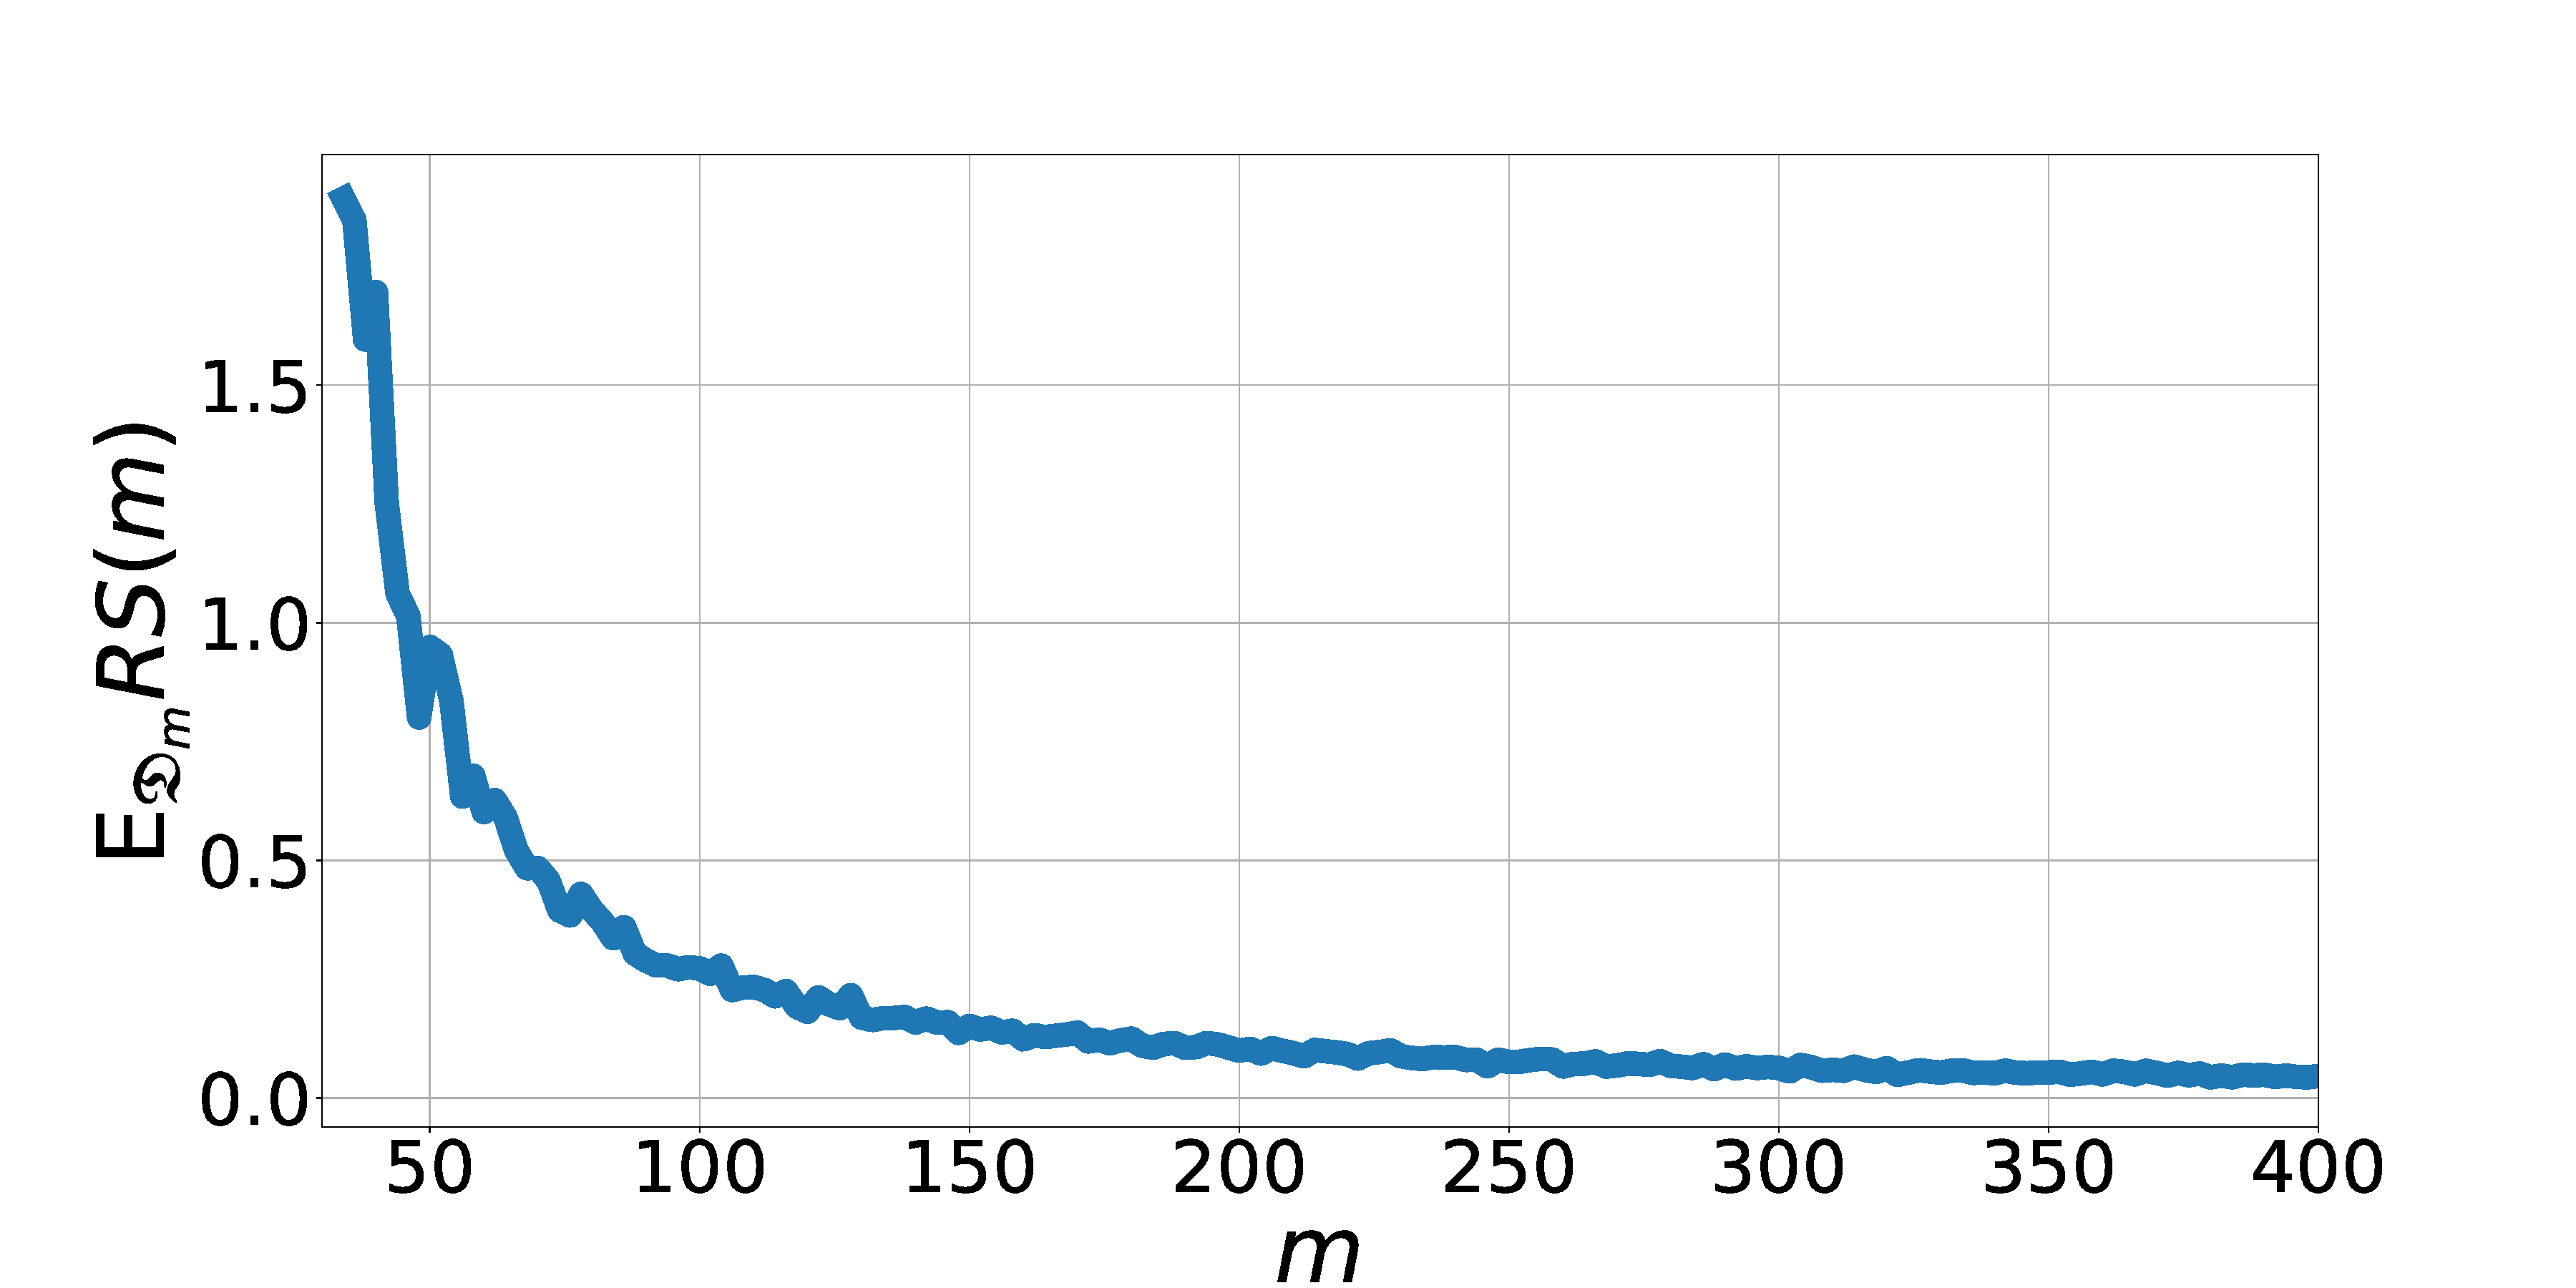
\includegraphics[width=0.49\textwidth]{results/samplesize/cross.pdf}
    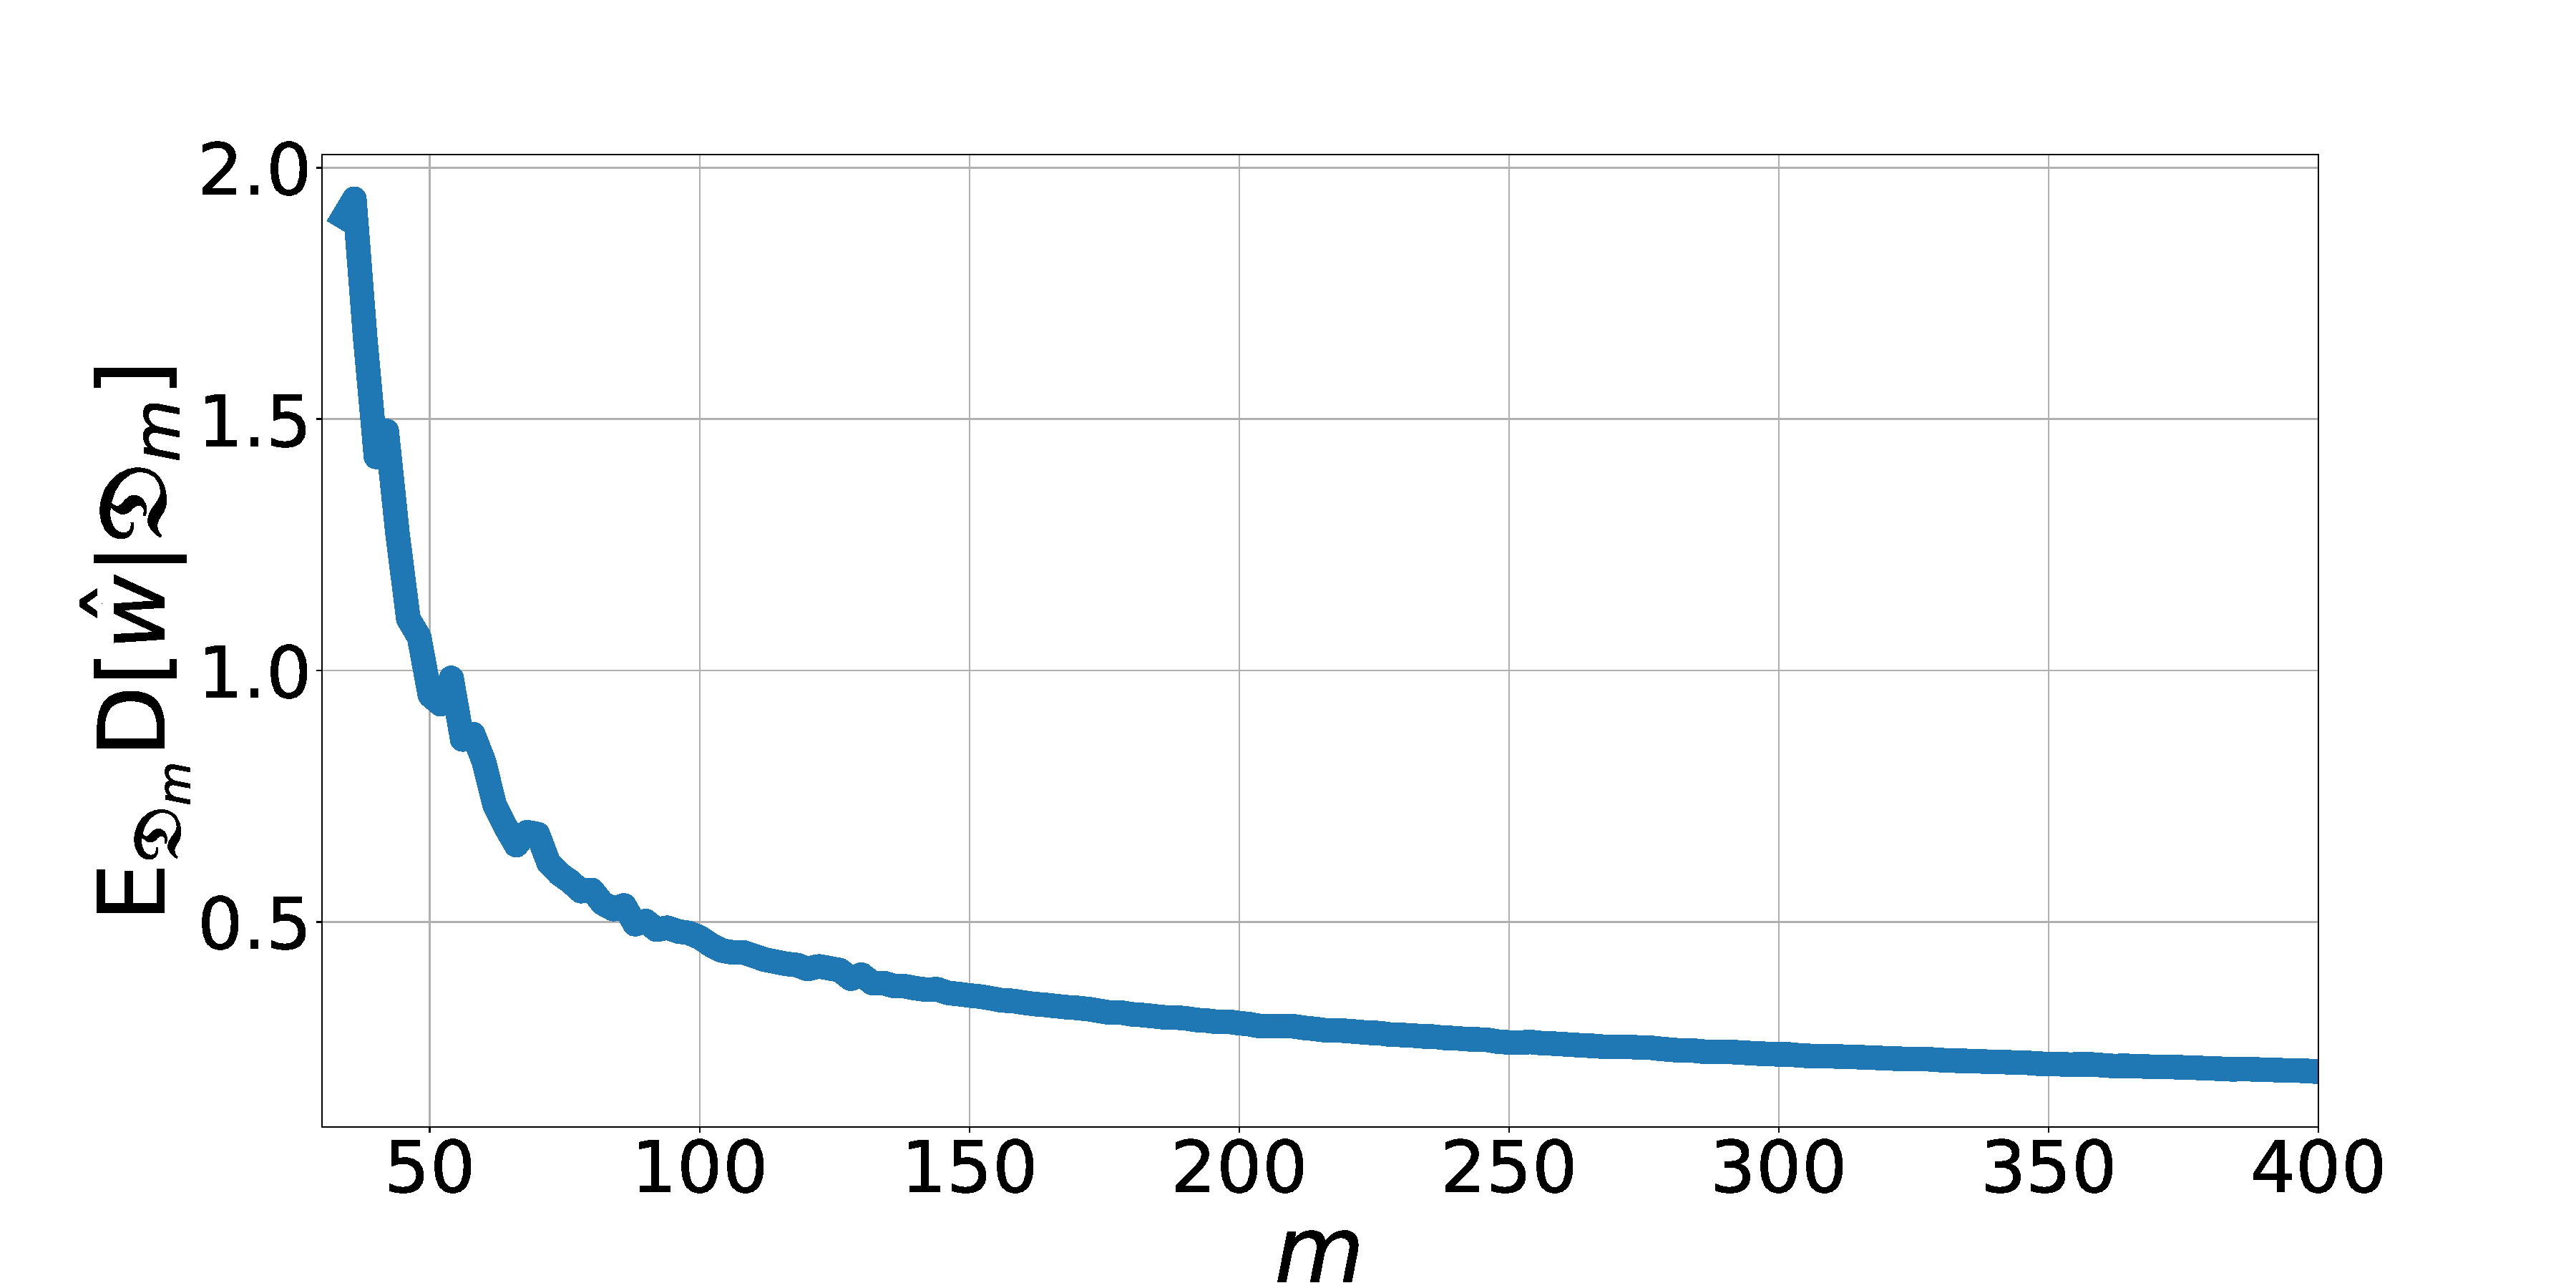
\includegraphics[width=0.49\textwidth]{results/samplesize/apvc.pdf}\\
    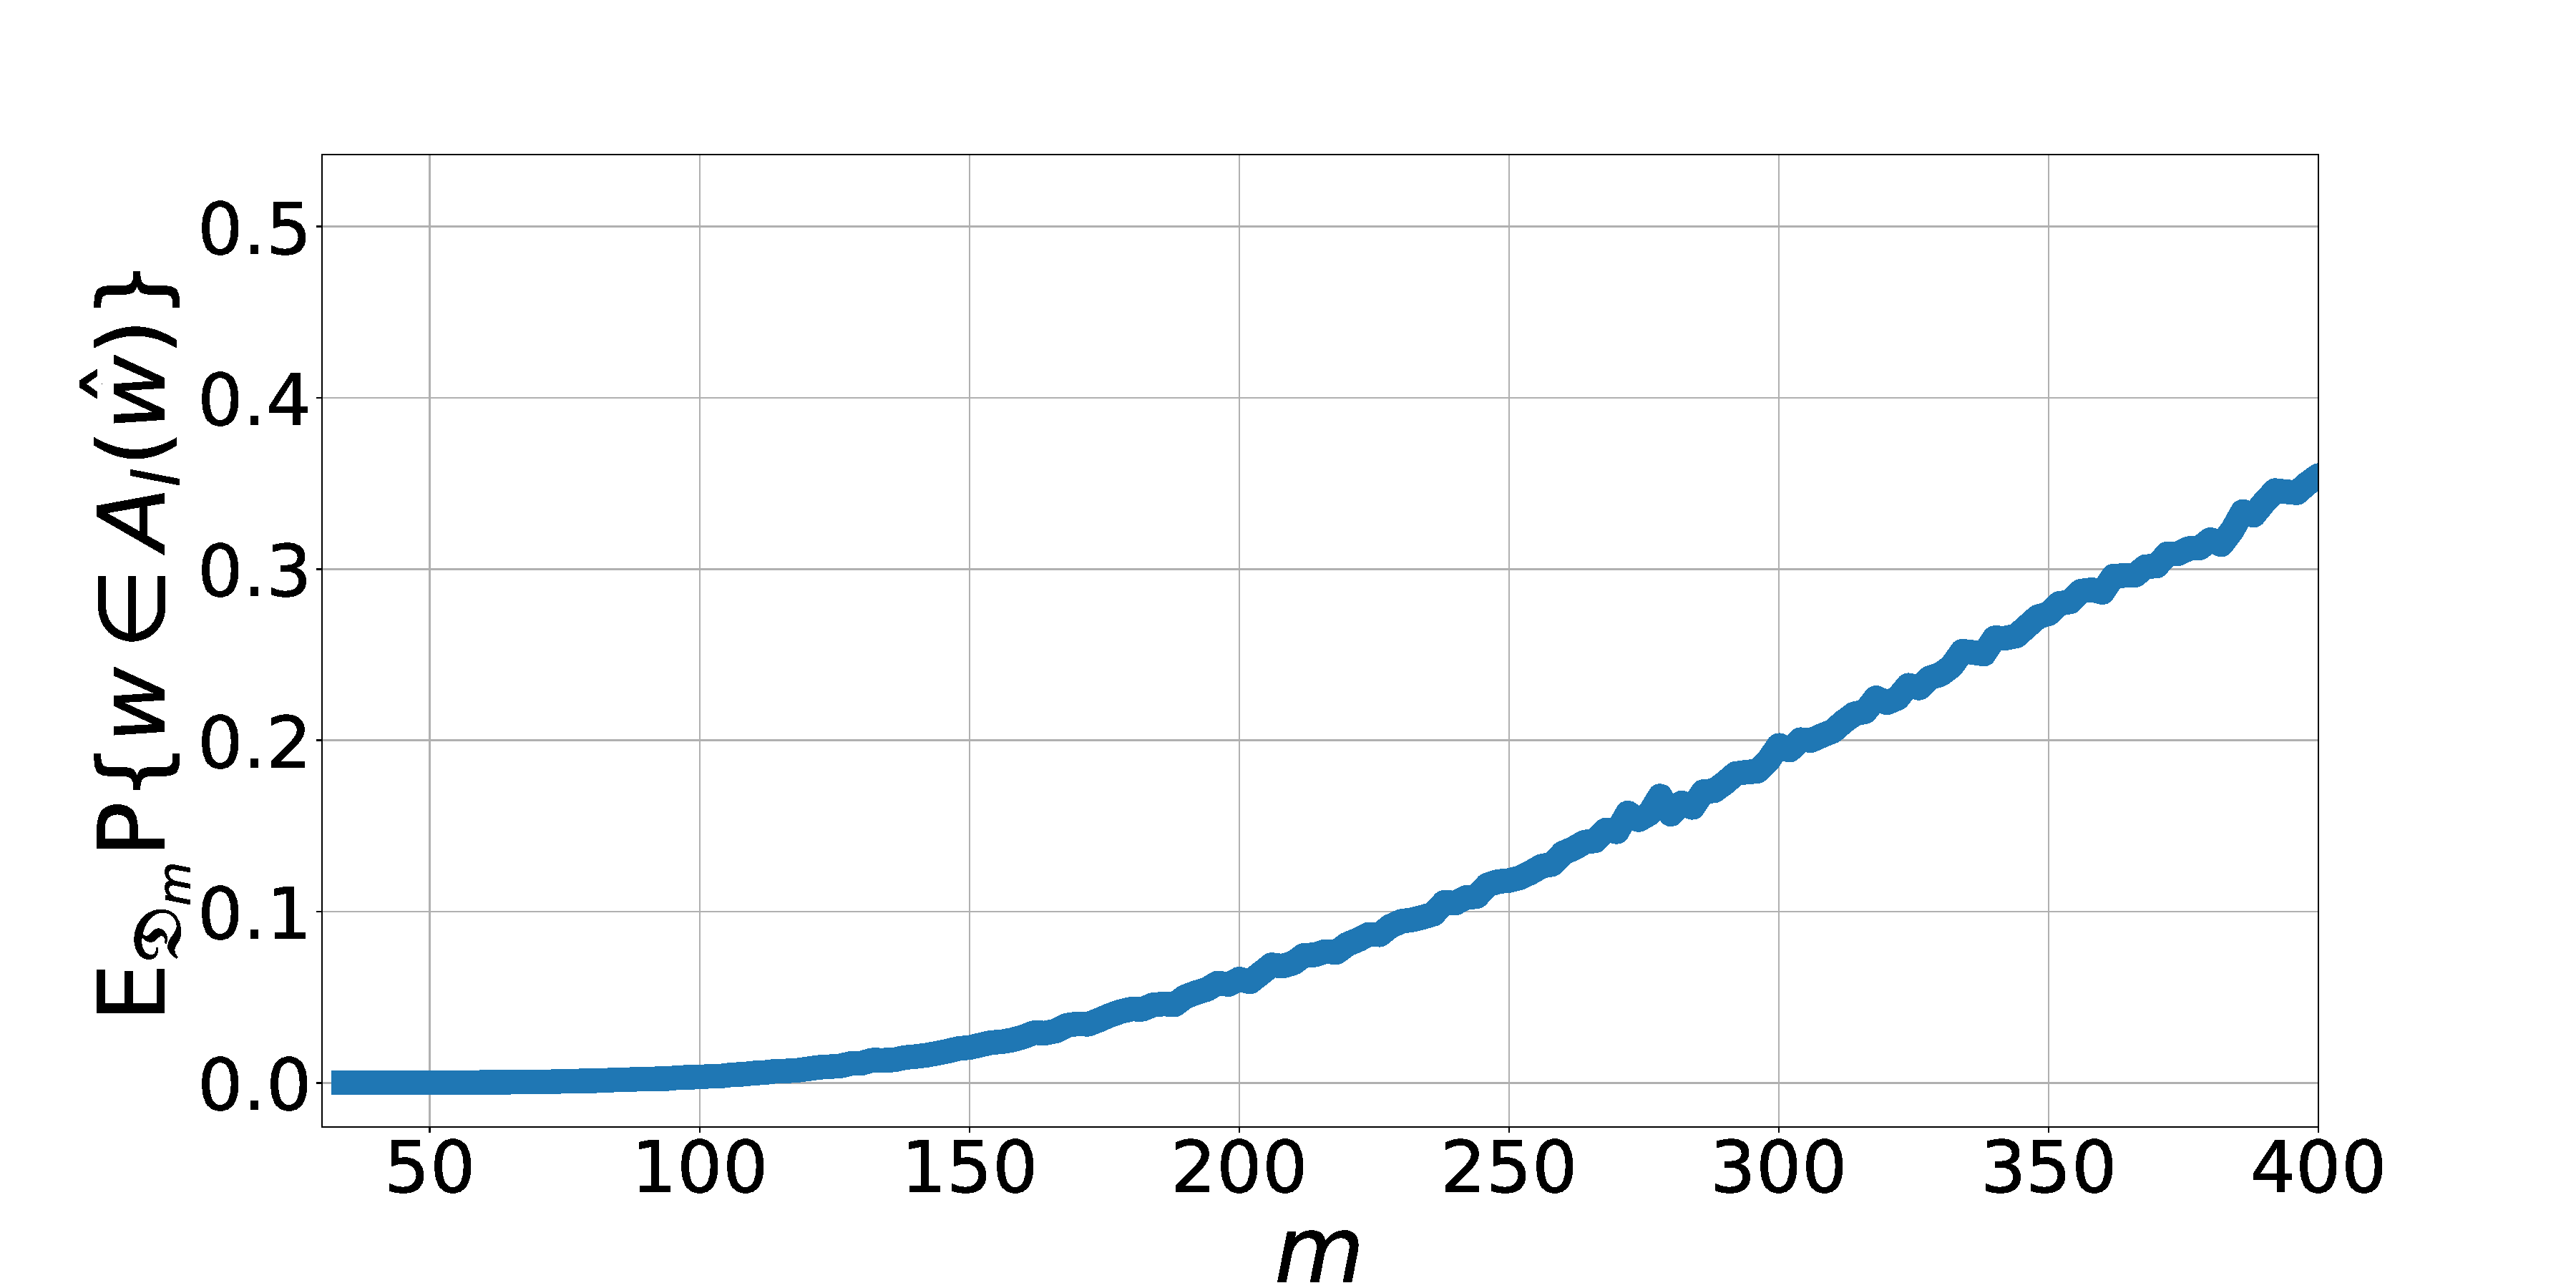
\includegraphics[width=0.49\textwidth]{results/samplesize/acc.pdf}
    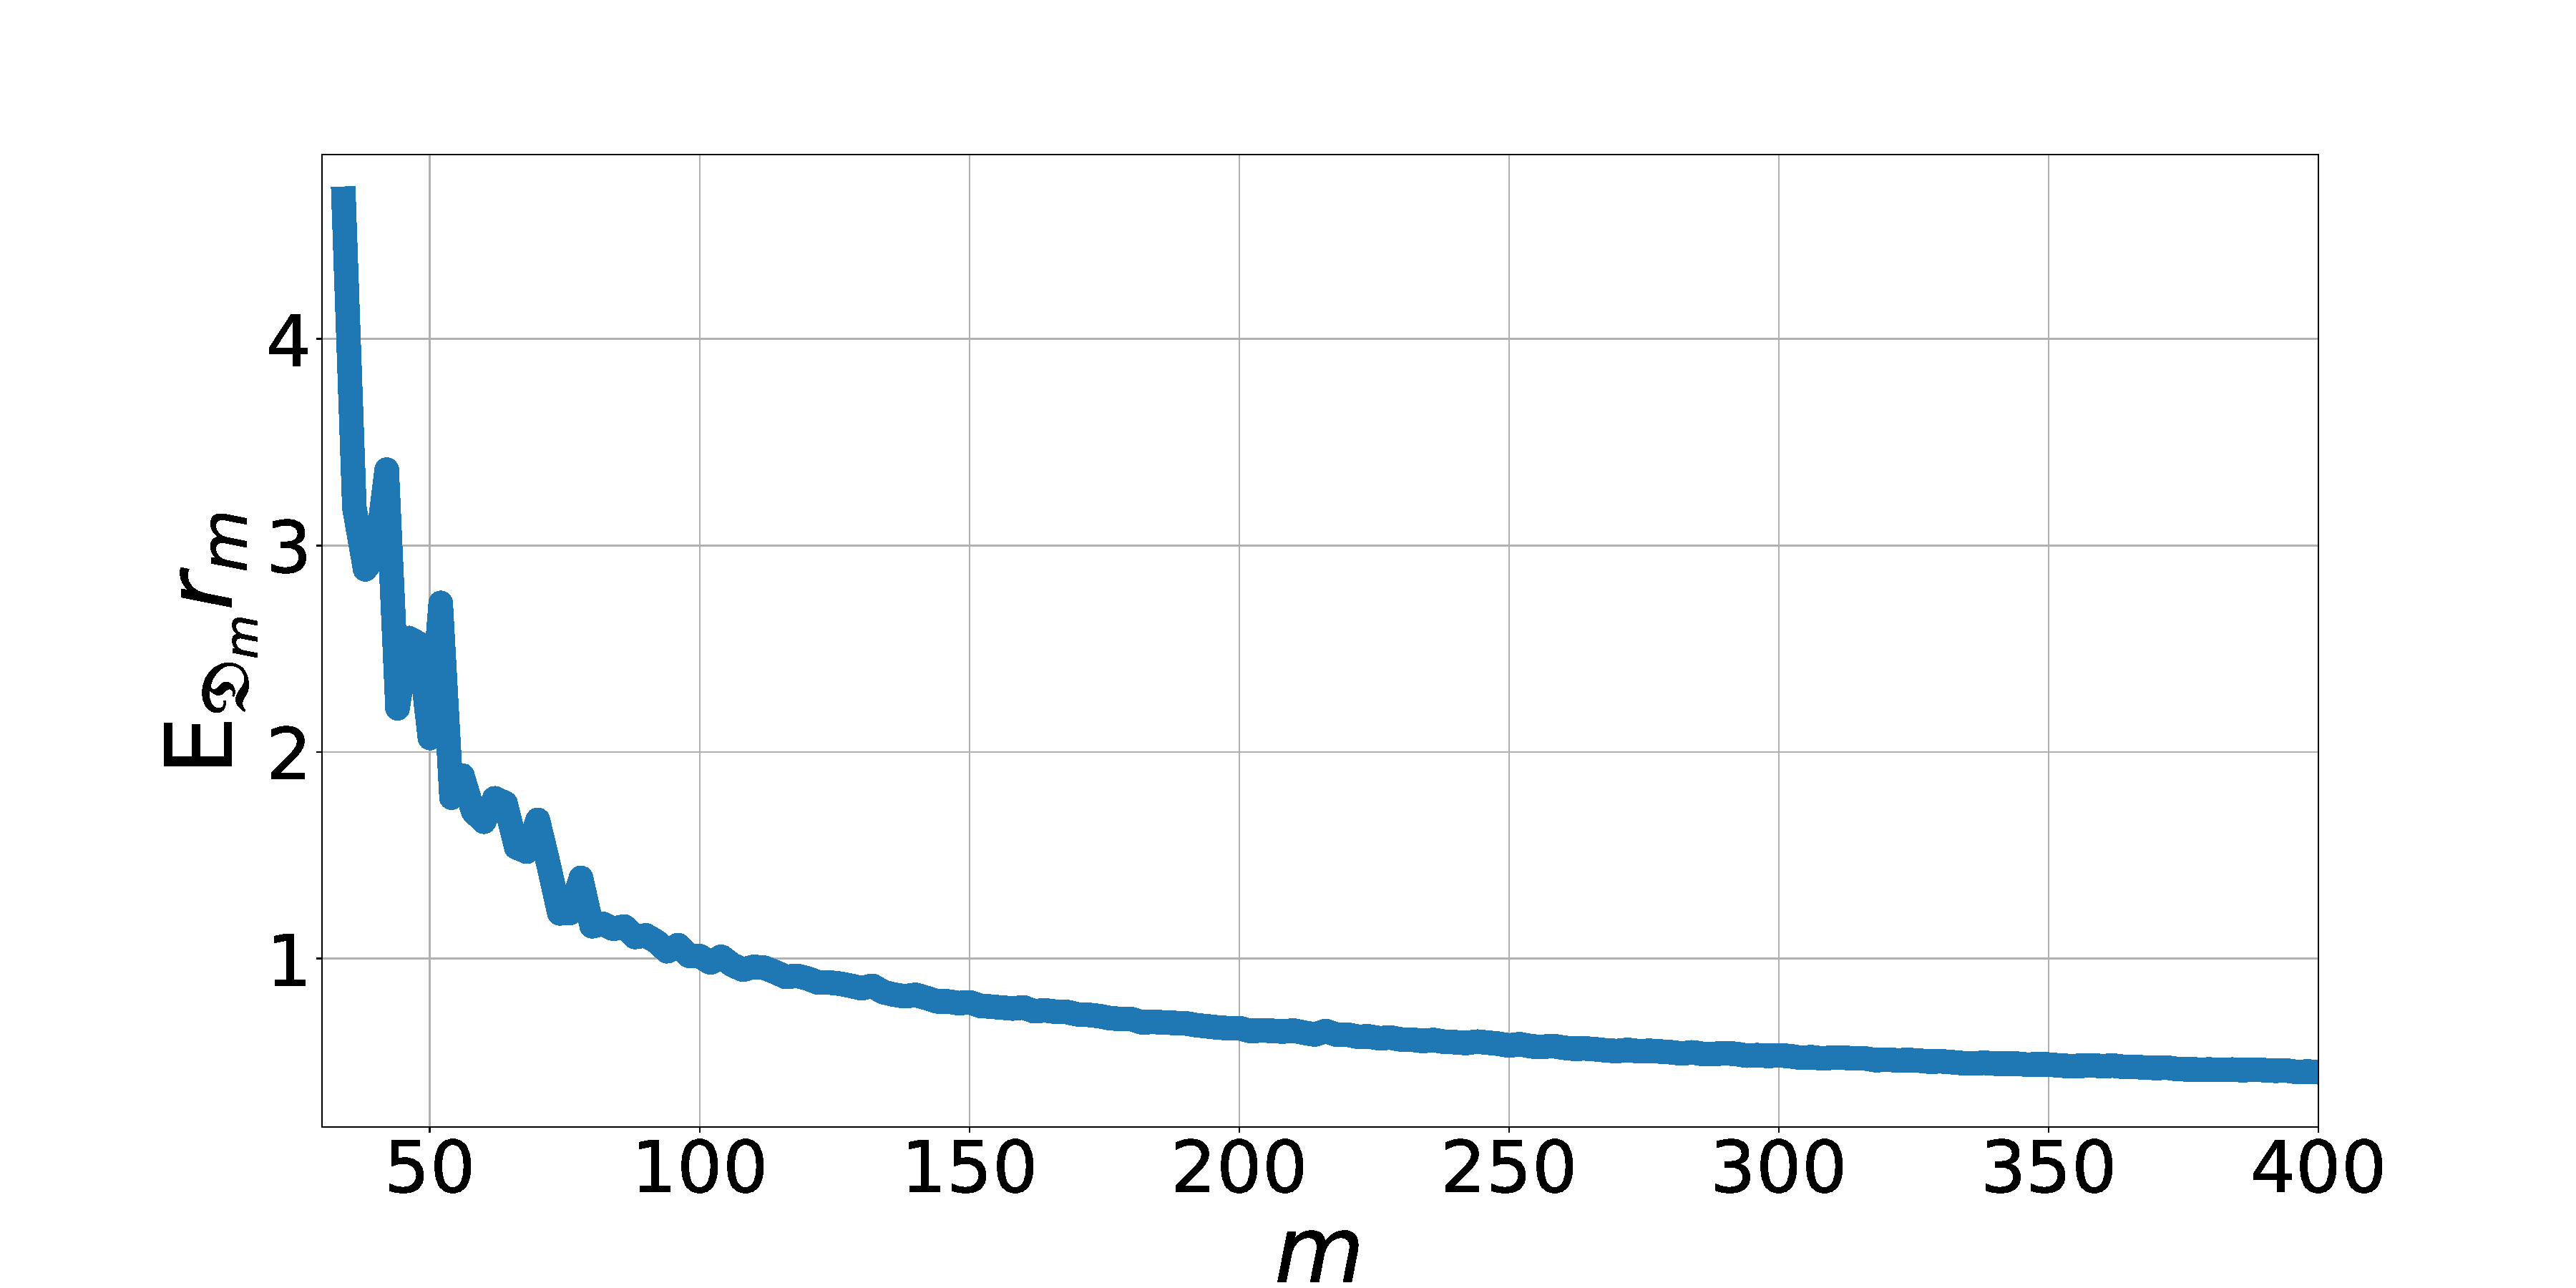
\includegraphics[width=0.49\textwidth]{results/samplesize/alc.pdf}\\
    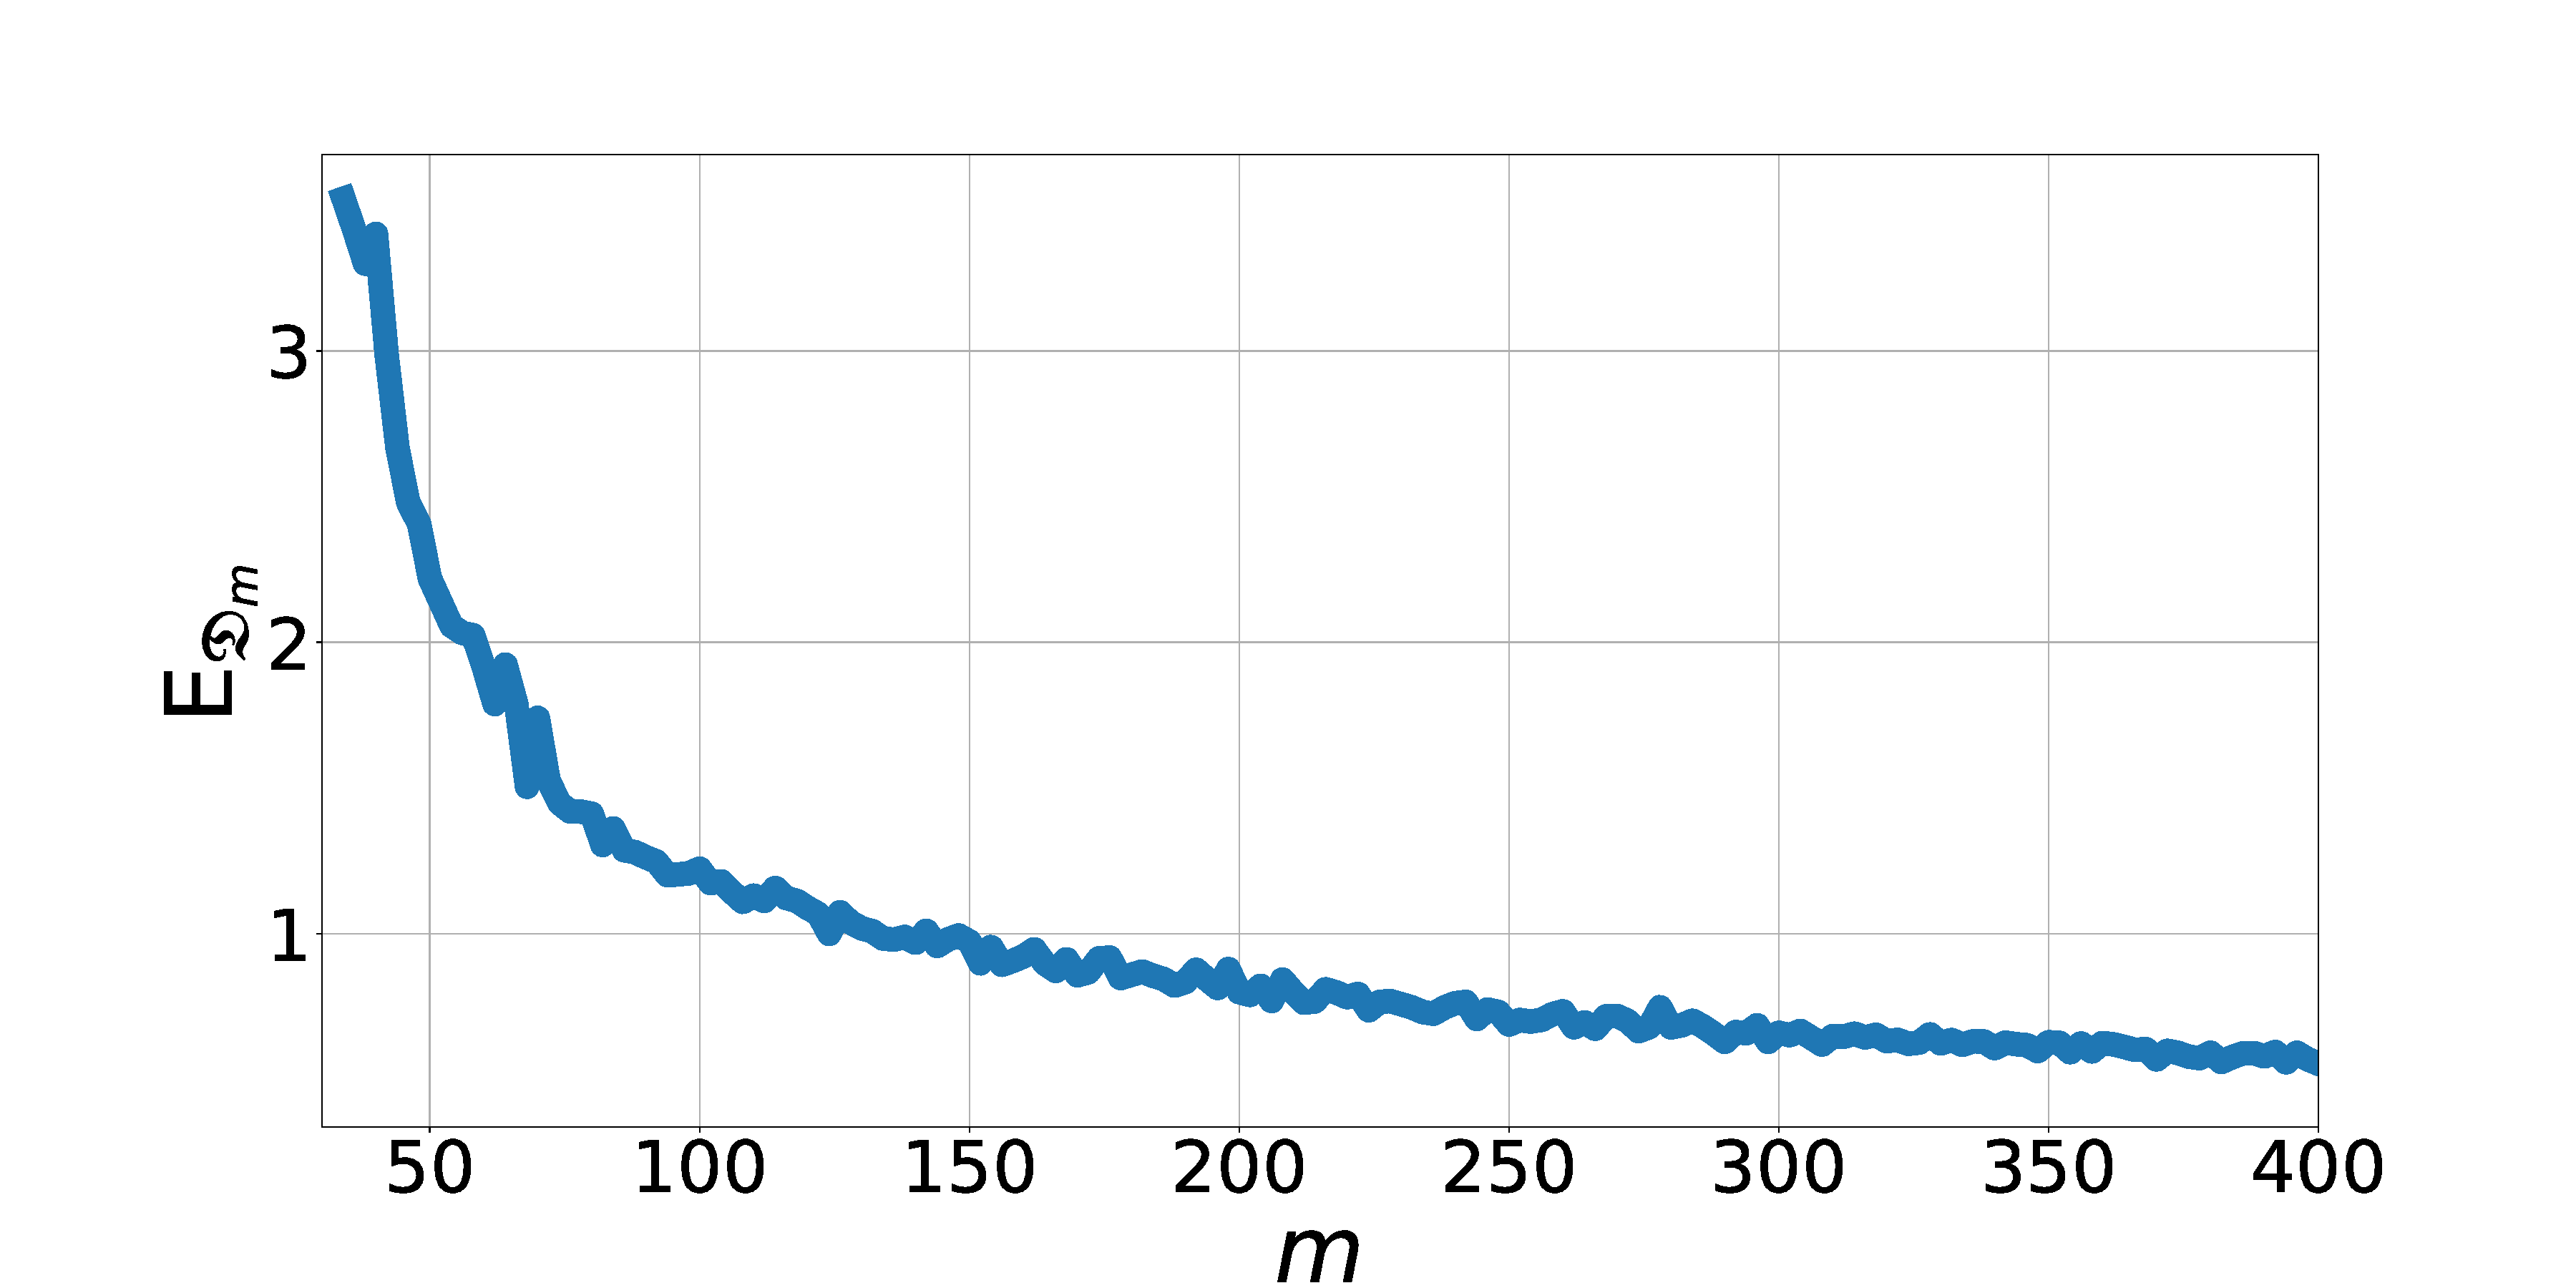
\includegraphics[width=0.49\textwidth]{results/samplesize/bootstrap.pdf}
    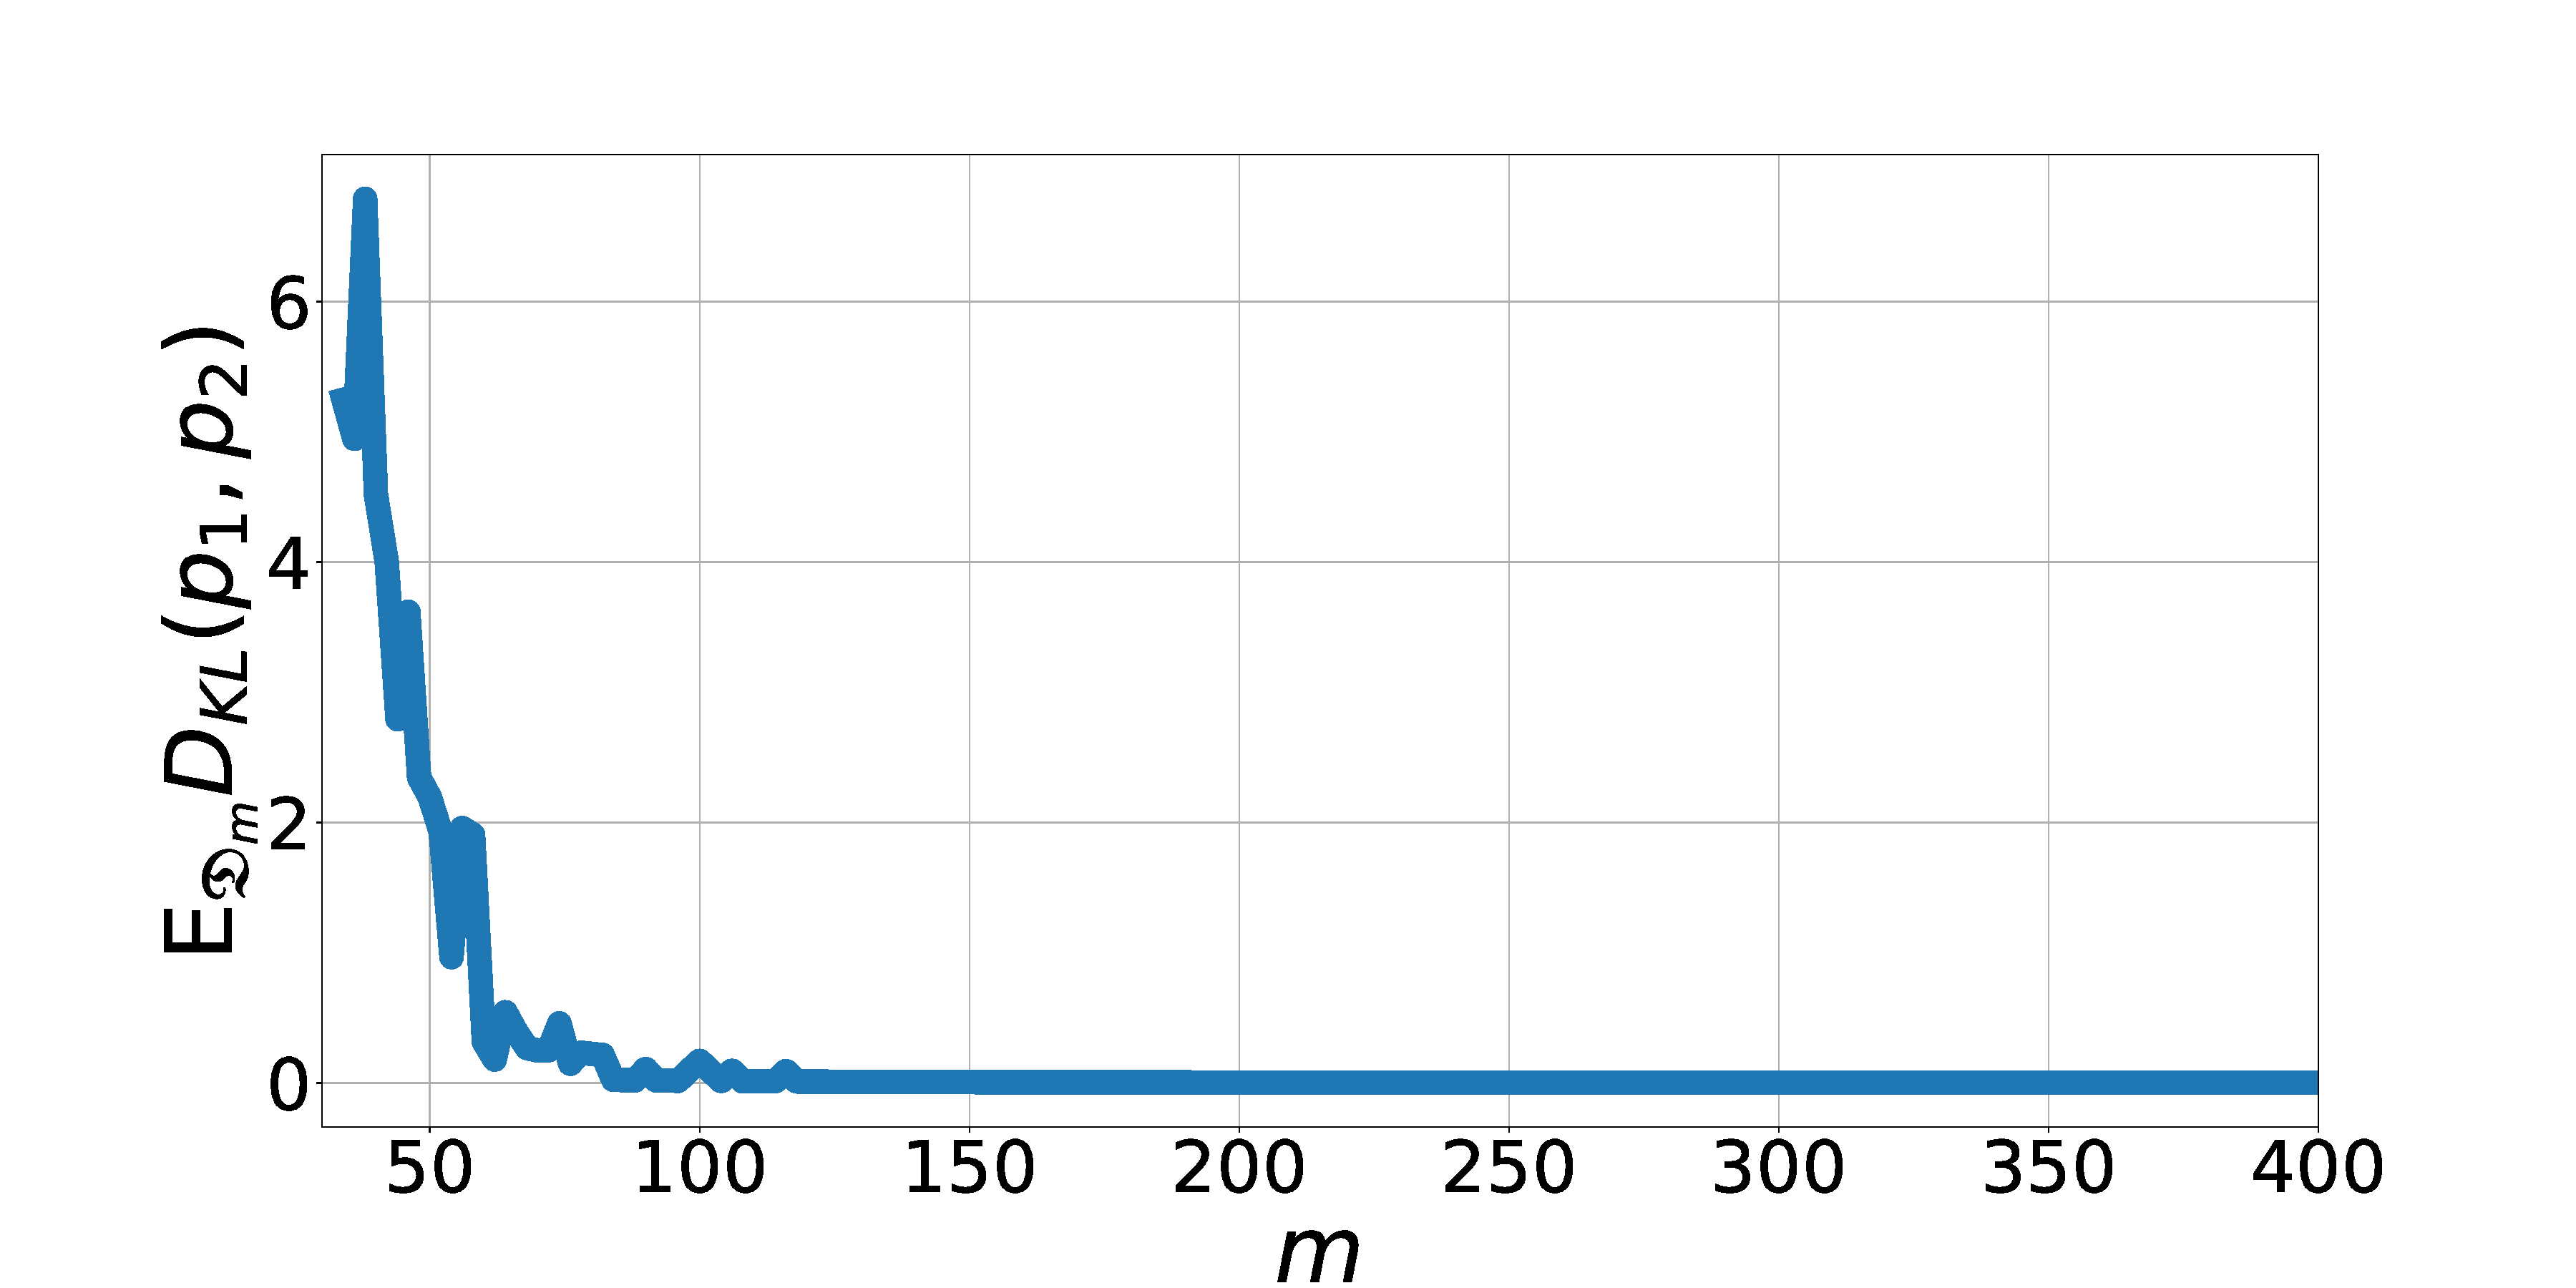
\includegraphics[width=0.49\textwidth]{results/samplesize/kl.pdf}\\
    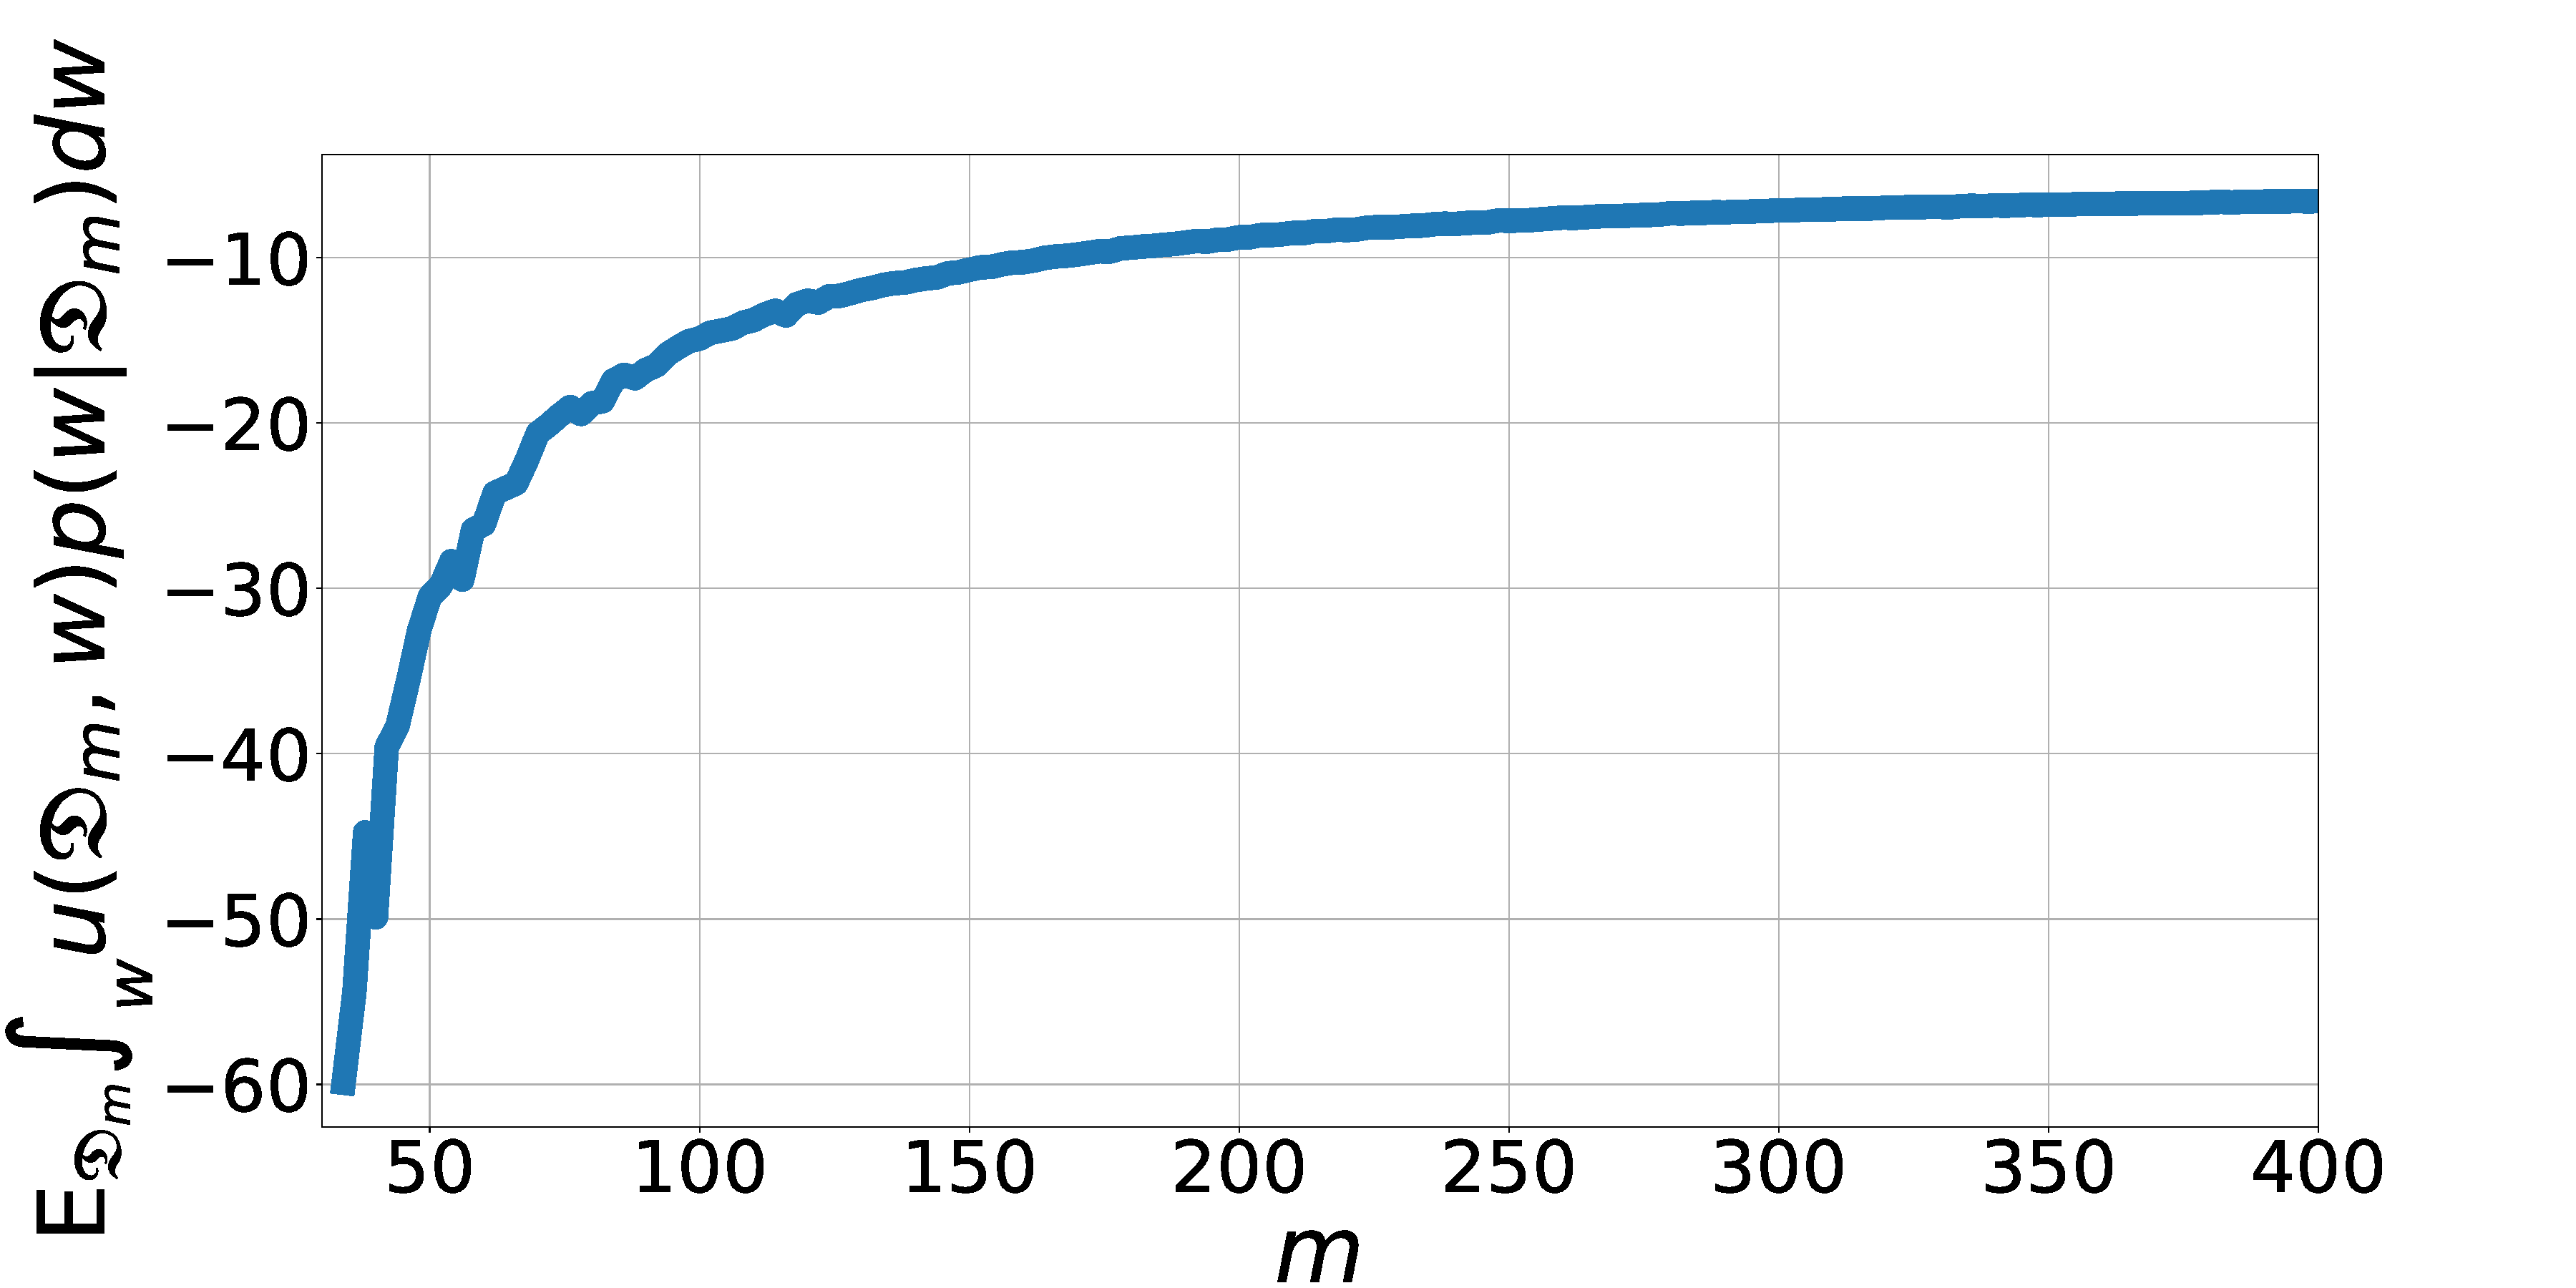
\includegraphics[width=0.49\textwidth]{results/samplesize/maxu.pdf}
    \caption{Зависимость статистических значений различных методов}
    \label{fig1}
\end{figure}

\begin{figure}[h!t]\center
    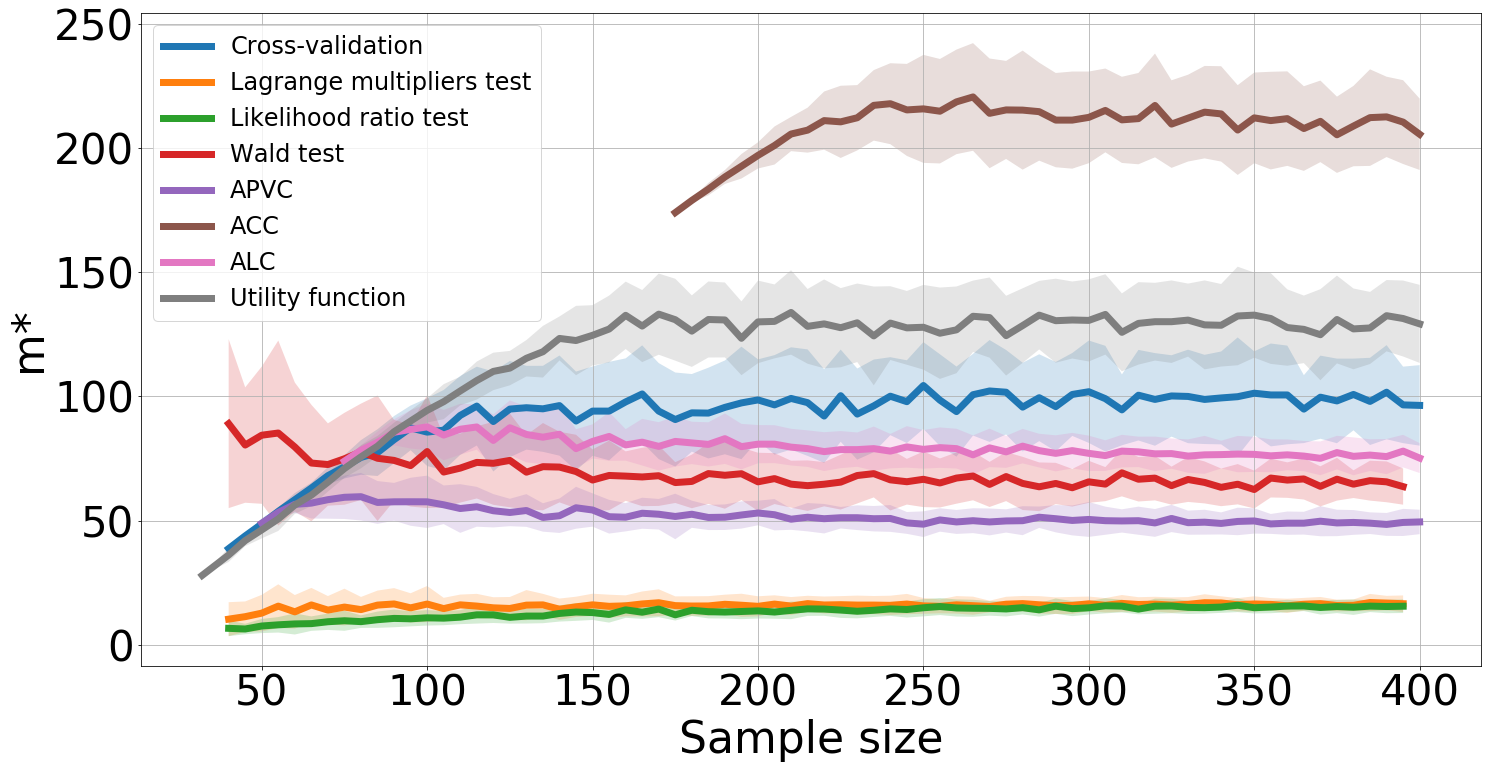
\includegraphics[width=0.85\textwidth]{results/samplesize/graphs.png}
    \caption{Анализ методов в зависимости от доступного размера выборки}
    \label{fig2}
\end{figure}

Рис.~\ref{fig1} демонстрирует зависимость статических значений каждого метода для разных выборок с фиксированным размером выборки~$m$. Пороговые значения для каждого метода устанавливаются экспертно, что позволяет контролировать различные статистические характеристики выборки. Рис.~\ref{fig1} показывает адекватность различных методов определения достаточного размера выборки. Представленные функции монотонны и асимптотически стремятся к константе.
На рис.~\ref{fig2} показаны результаты методов на выборках разных размера. Показано различие методов в дисперсии вычисленного~$m^*$. Анализируются различные методы в случае небольшого размера выборки. Все представленные методы сходятся, причем результат предсказания в асимптотике не зависит от доступного размера выборки~$m$.   

Небольшое значение дисперсии интерпретируется как вычислительная устойчивость рассмотренных методов. Показано, что некоторые методы не дают оценку достаточного размера выборки, если у них нет соответствующего размера выборки. Это значит, что они не эффективны с точки зрения прогноза, но могут быть использованы для ретроспективы и анализа уже проведенного эксперимента.

Анализируется оценка достаточного размера выборки в зависимости от гиперпараметров для байесовских методов, а также эврестических методов. Для анализа рассмотрена выборка {Boston Housing}.
Байесовские методы используют решающее правила над скалярной функцией для определения достаточного размера выборки. На рис.~\ref{fig1} показана зависимость скалярных функций от размера подвыборки. На рис.~\ref{fig1} показано, что эти функции монотонны. Тип поведения функции зависит от метода. Изменяя ограничения, установленные экспертно, можно изменить размер выборки, который будет соответствовать этим ограничениям.

\section{Кластеризация точек квазипериодических временных рядов}

Анализ физической активности человека производится при помощи мобильных телефонов, разумных часов~\cite{kwapisz2010, wang2014}. 
Эти устройства используют акселерометр, гироскоп и магнитометр. 
Цель данного исследования заключается в построения метода автоматической разметки и распознавании человеческой активности~\cite{Ignatov2015, Olivares2012, cinar2018}, а также поиска начала каждого действия~\cite{motrenko2015}. 
Примерами одного сегмента действия служит шаг, шаг бега, приседание, прыжок и др. 
Исследуются последовательности, которые состоят не менее чем из двух подряд идущих сегментов, которые соответствуют одному и тому жу типу человеческой активности.

\begin{figure}[h!t]\center
\subfloat[]
{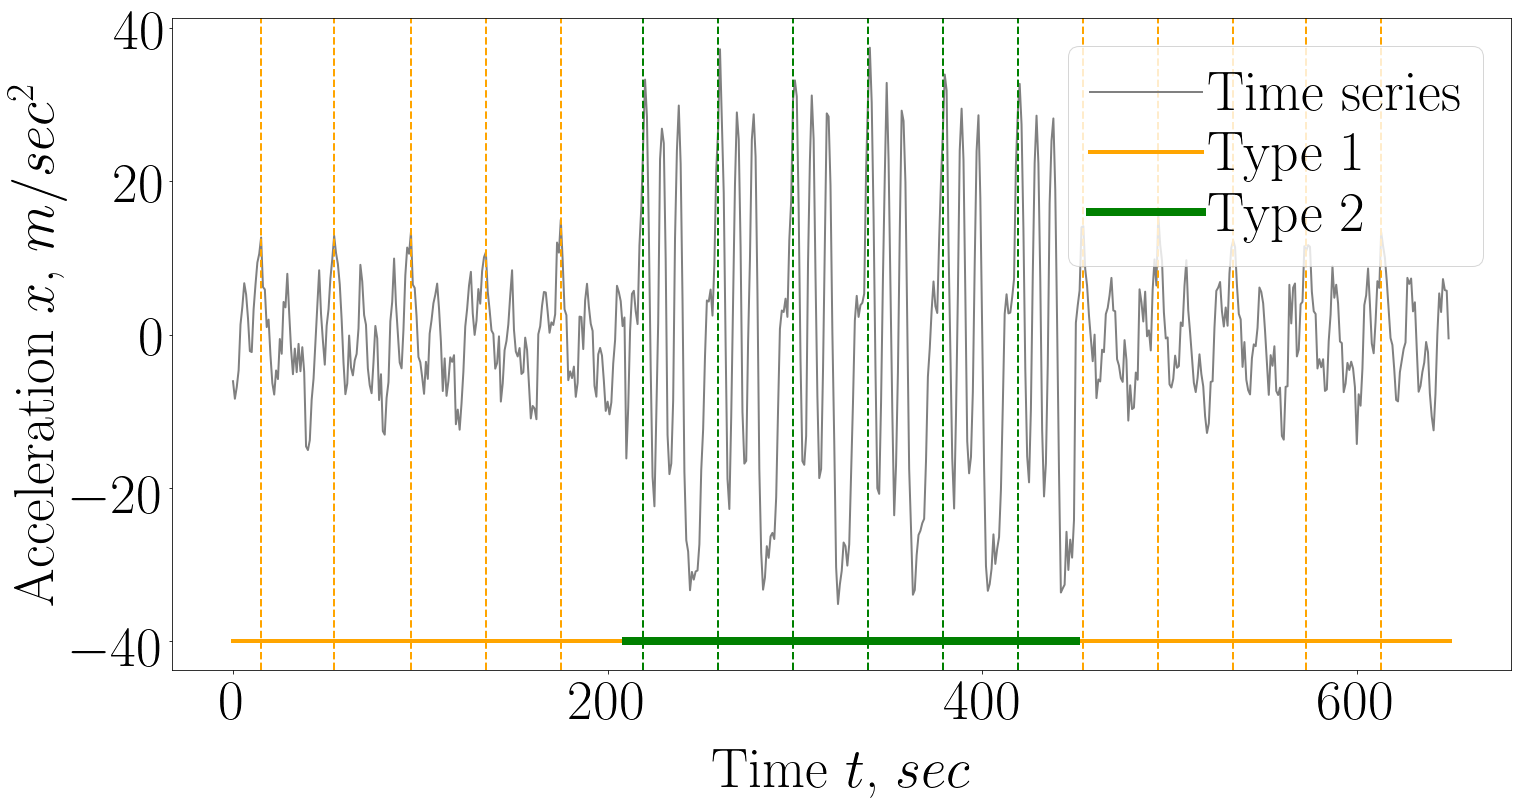
\includegraphics[width=0.5\textwidth]{results/series/example}\label{example:1}}
\subfloat[]
{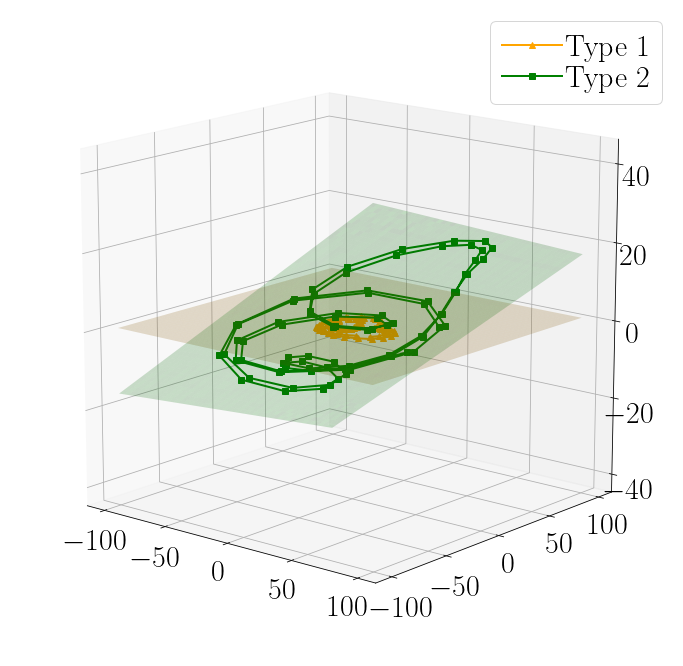
\includegraphics[width=0.5\textwidth]{results/series/example_phase}\label{example:2}}\\
\caption{Временной ряд, с разметкой на кластеры: a) временной ряд с ассесорской разметкой на кластеры и выделением начала квазипериодического сегмента; b) проекция фазовых траекторий на первые две главные компоненты}
\end{figure}

При классификации временных рядов значимую роль играет модель построения признакового пространства.
Объектом анализа и кластеризации является точка на оси времени. 
Решается задача кластеризации точек временного ряда. 
При \textit{кластеризации} каждой точке временного ряда ставится в соответствие метка из конечного множества меток. 
Каждая метка соответствует одному характерному физическому действию. \textit{Сегмент} это часть временного ряда, которая соответствует одному характерному физическому действию, например: шаг двумя ногами при ходьбе, или шаг двумя ногами при беге.
Последовательность сегментов, которые соответствуют одному физическому действия образуют \textit{цепочку} действий. 
Предполагается, что цепочка действий образует квазипериодическую последовательность значений временного ряда.
Последовательность точек~$\{b_t\}_{t=1}^{N}$ назовем \textit{квазипериодической} с периодом~$T$, если для всех~$t$ найдется~$\Delta$, такое что:
\[
\label{eq:int:1}
\begin{aligned}
b_t \approx b_{t+T+\Delta}, \quad \left|\Delta\right| \ll T.
\end{aligned}
\]
Пример кластеризации и разбиения ряда на сегменты показан на рис. \ref{example:1}. Данный ряд разбит на два характерных физических действия, которые обозначаются Type 1 и Type 2. Также данный ряд содержит в себе две квазипериодические цепочки действий.

Решение задачи кластеризации состоит из двух этапов. 
Во-первых, для получения признакового описания временного ряда предлагается алгоритм локальной аппроксимации временного ряда при помощи метода главных компонент~\cite{Shiglavsi1997}. 
Под \textit{локальной} аппроксимацией временного ряда подразумевается, что для признакового описания его точки используется не весь ряд, а только некоторая окрестность данной точки. 
В качестве признакового описания точки временного ряда рассматриваются две главные компоненты \textit{сегмента фазовой траектории} в окрестности данной точки.
На рис. \ref{example:2} показаны две первые главные компоненты \textit{фазовых траекторий}, а также проекция фазовых траекторий на эти компоненты.
Они соответствуют разным физическим действиям, которые обозначаются Type 1 и Type 2, внутри одного временного ряда.
Как видно, плоскости, порожденные главными компонентами не совпадают. 
Это говорит о том, что наблюдаются различные действия. 
Во-вторых, вводится функция расстояния в построенном пространстве признакового описания. 
Данная функция является расстояниям между двумя базисами некоторых подпространств внутри всего фазового пространства временного ряда.
На рис. \ref{example:2} данная функция является некоторым расстояниям между двумя плоскостями.
Получив расстояния между точками временного ряда, выполним кластеризацию данных точек.
Задача сегментации внутри каждого кластера решается при помощи метода, который рассмотрен в~\cite{motrenko2015}.

Для решения задачи кластеризации точек временного ряда вводятся предположения. 
Предполагается, что периоды различных сегментов различаются незначительно, причем известны минимальный и максимальный периоды сегмента и число различных сегментов внутри временного ряда. 
Также предполагается, что тип активности во времени не меняется часто, а также что фазовые траектории разных сегментов являются различными. 

Проверка и анализ метода кластеризации проводится на синтетической и реальной выборках.
Синтетическая выборка построена при помощи суммы нескольких первых членов ряда Фурье со случайными коэффициентами.
Эксперимент по сегментации временного ряда проводился на простых синусоидальных сигналах с произвольной амплитудой и частотой. 
Реальные данные получены при помощи мобильного акселерометра, который снимал показания во время некоторой физической активности человека. 

В~\cite{kwapisz2010} рассматривает метод построения признакового описания на основе экспертно-заданных порождающих функций.
В~\cite{lukashin2003} рассматривается метод построения признаков на основе гипотезы порождения данных. 
В~\cite{Ivkin2015} рассматривается комбинированное признаковое описание на основе данных методов. 
В~\cite{Katrutsa2015} рассматривается проблема построение признакового пространства и предлагается критерий избыточности выбранных признаков.

Работа~\cite{motrenko2015} является ближайшей работой по данной теме. Она заключается в поиске начала сегмента внутри квазипериодического сигнала, который состоит, только из одной цепочки действий. Этот метод основан на исследовании фазового пространства, а именно поиска устойчивой гиперплоскости, которая делит фазовое пространство на две равные части. В качестве начала сегмента выбираются точки, которые находятся близко к данной гиперплоскости. В~\cite{motrenko2015} предлагается выполнить проекцию фазового пространства на первые две главное компоненты, после чего провести устойчивую прямую, выделив начала каждого сегмента. 
Данный метод имеет недостаток в том, что позволяет находить начало только для временного ряда, который состоит из квазипериодического сигнала единственного типа.


Также близкой является работа~\cite{cinar2018}. Требуется найти периодическую структуру внутри ряда при помощи модели LSTM с модифицированным механизмом Attention. Предполагается, что механизм Attention будет давать максимальное значение score в точках, которые удаленны от данной на целое число периодов.

Задан временной ряд
\[
\label{eq:st:1}
\begin{aligned}
\textbf{x} \in \mathbb{R}^{N},
\end{aligned}
\]
где~$N$ число точек временного ряда. Он состоит из последовательности сегментов:
\[
\label{eq:st:2}
\begin{aligned}
\textbf{x} = [\textbf{v}_1, \textbf{v}_2, \ldots, \textbf{v}_M],
\end{aligned}
\]
где~$\textbf{v}_i$ некоторый сегмент из множества сегментов~$\mathbf{V}$, которые встречаются в данном ряде. 
Причем для всех~$i$ либо~$[\textbf{v}_{i-1},\textbf{v}_{i}]$ либо~$[\textbf{v}_{i},\textbf{v}_{i+1}]$  является цепочкой действий. Пусть множество~$\mathbf{V}$ удовлетворяет свойствам:

\[
\label{eq:st:3}
\begin{aligned}
\left|\mathbf{V}\right| = K, \quad \textbf{v} \in \mathbf{V} \left|\textbf{v}\right| \leq T,
\end{aligned}
\]
где~$\left|\mathbf{V}\right|$ число различных действий в множестве сегментов~$\mathbf{V},$~$\left|\textbf{v}\right|$ длина сегмента, а~$K$ и~$T$ это число различных действий во временном ряде и длина максимального сегмента соответсвенно.

Рассматривается отображение
\[
\label{eq:st:4}
\begin{aligned}
a : t \to \mathbb{Y} = \{1,\ldots, K\}, 
\end{aligned}
\]
где~$t \in \{1,\ldots, N\}$ некоторый момент времени, на котором задан временной ряд.
Требуется, чтобы отображение~$a$ удовлетворяло свойствам:

\[
\label{eq:st:5}
\begin{aligned}
\begin{cases}
    a\left(t_1\right) = a\left(t_2\right), &  \text{если в моменты } t_1, t_2 \text{ совершается один тип действий},\\
    a\left(t_1\right) \not= a\left(t_2\right), &  \text{если в моменты } t_1, t_2 \text{ совершаются разные типы действий.}
\end{cases}
\end{aligned}
\]

Пусть задана некоторая асессорская разметка временного ряда:
\[
\label{eq:st:6}
\begin{aligned}
\textbf{y} \in \{1,\ldots,K\}^{N}.
\end{aligned}
\]
Тогда ошибка алгоритма~$a$ на временном ряде~$\textbf{x}$ представляется в виде:
\[
\label{eq:st:7}
\begin{aligned}
S = \frac{1}{N}\sum_{t=1}^{N}[y_t = a\left(t\right)],
\end{aligned}
\]
где~$t$ --- момент времени,~$y_t$ асессорская разметка~$t$-го момента времени для заданого временного ряда.


\paragraph{Кластеризация точек в фазовом пространстве.}
Рассмотрим фазовую траекторию временного ряда~$\textbf{x}$:
\[
\label{eq:cl:1}
\begin{aligned}
\mathbf{H} = \{\textbf{h}_t| \textbf{h}_t = [x_{t-T}, x_{t-T+1}, \ldots, x_{t}], T\leq t\leq N\},
\end{aligned}
\]
где~$\textbf{h}_t$ --- точка фазовой траектории.

Информация об длине максимального сегмента~$T$ внутри временного ряда позволяет разбить фазовую траекторию на сегменты из~$2T$ векторов:
\[
\label{eq:cl:2}
\begin{aligned}
\mathbf{S} = \{\textbf{s}_t| \textbf{s}_t = [\textbf{h}_{t-T}, \textbf{h}_{t-T+1}, \ldots, \textbf{h}_{t+T-1}], T\leq t\leq N-T\},
\end{aligned}
\]
где~$\textbf{s}_t$ --- это сегмент фазовой траектории. Данные сегменты имеют всю локальную информацию об временном ряде, так как содержит всю информацию на периоде до момента времени~$t$ и информацию о периоде после момента времени~$t$.

В качестве признакового описания точки временного ряда~$t$ рассматриваются главные компоненты~$\textbf{W}_t$ для~$T\text{-мерных}$ сегментов~$\textbf{s}_t$. Сегмент~$\textbf{s}_t$ проекцируется на подпространство размерности два при помощи метода главных  компонент~$\textbf{z}_t = \textbf{W}_t\textbf{s}_t$. Получаем:

%Каждое~$T\text{-мерное}$ подпространство~$\textbf{s}_t$ проектируется на подпространство значительно меньшей размерности при помощи метода главных  компонент~$\textbf{z}_t = \textbf{W}_t\textbf{s}_t$. Получим представление базисных векторов~$\textbf{W}_t$, а также собственные числа, которые соответствуют данным базисным векторам каждого подпространства~$\textbf{s}_t$ в~$T\text{-мерном}$ пространстве:
\[
\label{eq:cl:3}
\begin{aligned}
\mathbf{W} = \{\textbf{W}_t| \textbf{W}_t = [\lambda^1_t\textbf{w}^1_t, \lambda^2_t\textbf{w}^2_t]\}, \quad \bm{\Lambda} = \{\bm{\lambda}_t| \bm{\lambda}_t=[\lambda^1_t, \lambda^2_t]\},
\end{aligned}
\]
где~$[\textbf{w}^1_t, \textbf{w}^2_t]$ и~$[\lambda^1_t, \lambda^2_t]$ это базисные векторы и соответствующие им собственные для сегмента фазовой траектории~$\textbf{s}_t$.

Для кластеризации точек временного ряда рассмотрим функцию расстояния между элементами~$\mathbf{W}_{t_1},\mathbf{W}_{t_2}$:
\[
\label{eq:cl:4}
\begin{aligned}
\rho\left(\textbf{W}_1, \textbf{W}_2\right) = \max\left(\max_{\textbf{e}_2 \in \textbf{W}_2} d_{1}\left(\textbf{e}_2\right), \max_{\textbf{e}_1 \in \textbf{W}_1} d_{2}\left(\textbf{e}_1\right)\right),
\end{aligned}
\]
где ~$\textbf{e}_i$ это базисный вектор пространства~$\textbf{W}_i,$ а~$d_i\left(\textbf{e}\right)$ является расстоянием от вектора~$\textbf{e}$ до пространства~$\textbf{W}_i$.

\begin{comment}
\begin{theorem}
Пусть задано множество подпространств~$\mathbb{W}$ пространства~$\mathbb{R}^{n}$. Каждое подпространство которого задается базисом~$\mathbf{W}_i\in \mathbf{W}$, тогда функция расстояния~$\rho\left(\textbf{W}_1, \textbf{W}_2\right)$ является метрикой заданой на множестве базисов~$\mathbf{W}$:
\[
\begin{aligned}
\rho\left(\textbf{W}_1, \textbf{W}_2\right) = \max\left(\max_{\textbf{e}_2 \in \textbf{W}_2} d_{1}\left(\textbf{e}_2\right), \max_{\textbf{e}_1 \in \textbf{W}_1} d_{2}\left(\textbf{e}_1\right)\right),
\end{aligned}
\]
где~$\textbf{e}_i$ это базисный вектор из~$\textbf{W}_i$, a~$d_i\left(\textbf{e}\right)$ является расстоянием от вектора~$\textbf{e}$ до пространства заданого базисом~$\textbf{W}_i$.
\end{theorem}

В силу теоремы \ref{th:1} функция расстояния (\ref{eq:cl:4}) является метрикой, доказательство данной теоремы представлено в приложении \ref{ProofTheorem1}. 
\end{comment}

В случае, когда все подпространства~$\textbf{W}_t$ имеют размерность два, расстояние~$\rho\left(\textbf{W}_1, \textbf{W}_2\right)$ имеет интерпретацию:

\[
\label{eq:cl:5}
\begin{aligned}
\rho\left(\textbf{W}_1, \textbf{W}_2\right) = \max_{\{\textbf{a},\textbf{b},\textbf{c}\} \subset \textbf{W}_1\cup \textbf{W}_2 } V\left(\textbf{a},\textbf{b},\textbf{c}\right), 
\end{aligned}
\]
где~$\textbf{W}_1\cup\textbf{W}_2$ это объединение базисных векторов первого и второго пространства,~$V\left(\textbf{a},\textbf{b},\textbf{c}\right)$ --- объем параллелепипеда построенного на векторах~$\textbf{a}, \textbf{b}, \textbf{c}$, которые являются столбцами матрицы~$\textbf{W}_1\cup\textbf{W}_2$.


Рассмотрим расстояние между собственными числами:
\[
\label{eq:cl:6}
\begin{aligned}
\rho\left(\bm{\lambda}_1, \bm{\lambda}_2\right) = \sqrt[]{\left(\bm{\lambda}_1 - \bm{\lambda}_2\right)^{\mathsf{T}}\left(\bm{\lambda}_1 - \bm{\lambda}_2\right)}.
\end{aligned}
\]
%Функция расстояния~$\rho\left(\bm{\lambda}_1, \bm{\lambda}_2\right)$ является метрикой в пространстве~$\mathbb{R}^2$.
%Матрица попарных расстояний между базисными векторами~$\textbf{M}_{\text{c}}$ и матрица попарных расстояний между собственными значениями~$\textbf{M}_{\text{l}}$ для временного ряда~$\textbf{x}$:
%\[
%\label{eq:cl:8}
%\begin{aligned}
%\textbf{M}_{\text{c}} = [0, 1]^{N\times N}, \quad \textbf{M}_{\text{l}} = [0, 1]^{N\times N}.
%\end{aligned}
%\]
Используя выражения (\ref{eq:cl:5}-\ref{eq:cl:6}) введем расстояние между двумя точками~$t_1, t_2$ временного ряда, а также рассмотрим матрицу попарных расстояний~$\textbf{M}$ между точками данного ряда:
\[
\label{eq:cl:9}
\begin{aligned}
\rho\left(t_1, t_2\right) = \rho\left(\textbf{W}_1, \textbf{W}_2\right) + \rho\left(\bm{\lambda}_1, \bm{\lambda}_2\right), \quad \textbf{M} =  \mathbb{R}^{N\times N},
\end{aligned}
\]
где %~$\rho\left(t_1, t_2\right)$ является метрикой, так как является суммой двух метрик,
матрица~$\textbf{M}$ является матрицей попарных расстояний между всеми парами точек~$t$ временного ряда~$\textbf{x}$.
Используя матрицу попарных расстояний~$\textbf{M}$ выполним кластеризацию моментов времени~$t$ временного ряда \eqref{eq:st:4}:

\[
\label{eq:cl:10}
\begin{aligned}
a : t \to \{1,\ldots, K\}, 
\end{aligned}
\]
где~$t$ некоторый момент времени временного ряда~$\textbf{x}$.

\section{Анализ фазовых траекторий в задаче кластеризации}
Для анализа свойств предложенного алгоритма кластериизации проведен вычислительный эксперимент в котором кластеризация точек временного ряда проводилась используя матрицы попарных расстояний~$(\ref{eq:cl:9})$.

В качестве данных использовались две выборки временных рядов, которые описаны в таблице \ref{table_1}. 
Выборка Physical Motion это реальные временные ряды полученные при помощи мобильного акселерометра. 
Синтетические временные ряды построены при помощи нескольких первых слагаемых ряда Фурье со случайными коэффициентами из стандартного нормального распределения. 
Генерация данных состояла из двух этапов. 
На первом этапе генерировались короткие сегменты~$\textbf{v}$ для построения множества~$\mathbf{V}$. 
Вторым этапом генерации выборки~$\textbf{x}$ является случайным процессом:
\[
\label{eq:exp:1}
\begin{aligned}
\textbf{x} = [\textbf{v}_{1}, \textbf{v}_{2}, \ldots, \textbf{v}_{M}] + \bm{\varepsilon}, \quad \begin{cases}
    \textbf{v}_{1} \sim \mathcal{U}\left(\mathbf{V}\right),\\
    \textbf{v}_{i} = \textbf{v}_{i - 1}, & \text{с вероятностью} \frac{3}{4}\\
    \textbf{v}_{i} \sim \mathcal{U}\left(\mathbf{V}\right), & \text{с вероятностью} \frac{1}{4}
\end{cases},
\end{aligned}
\]
где~$\mathcal{U}\left(\mathbf{V}\right)$ --- равномерное распределение на объектах из~$\mathbf{V},$ а~$\bm{\varepsilon}$ является шумом из нормального распределения.

\begin{table}[h!t]
\begin{center}
\caption{Описание временных рядов в эксперименте кластеризации точек временного ряда}
\label{table_1}
\begin{tabular}{|c|c|c|c|}
\hline
	Ряд,~$\textbf{x}$ &Длина ряда,~$N$& Число сегментов,~$K$&Длина сегмента,~$T$\\
	\hline
	\multicolumn{1}{|l|}{Physical Motion 1}
	& 900& 2& 40\\
	\hline
	\multicolumn{1}{|l|}{Physical Motion 2}
	& 900& 2& 40\\
	\hline
	\multicolumn{1}{|l|}{Synthetic 1}
	& 2000& 2& 20\\
	\hline
	\multicolumn{1}{|l|}{Synthetic 2}
	& 2000& 3& 20\\
\hline

\end{tabular}
\end{center}
\end{table}

\begin{figure}[h!t]\center
\subfloat[]
{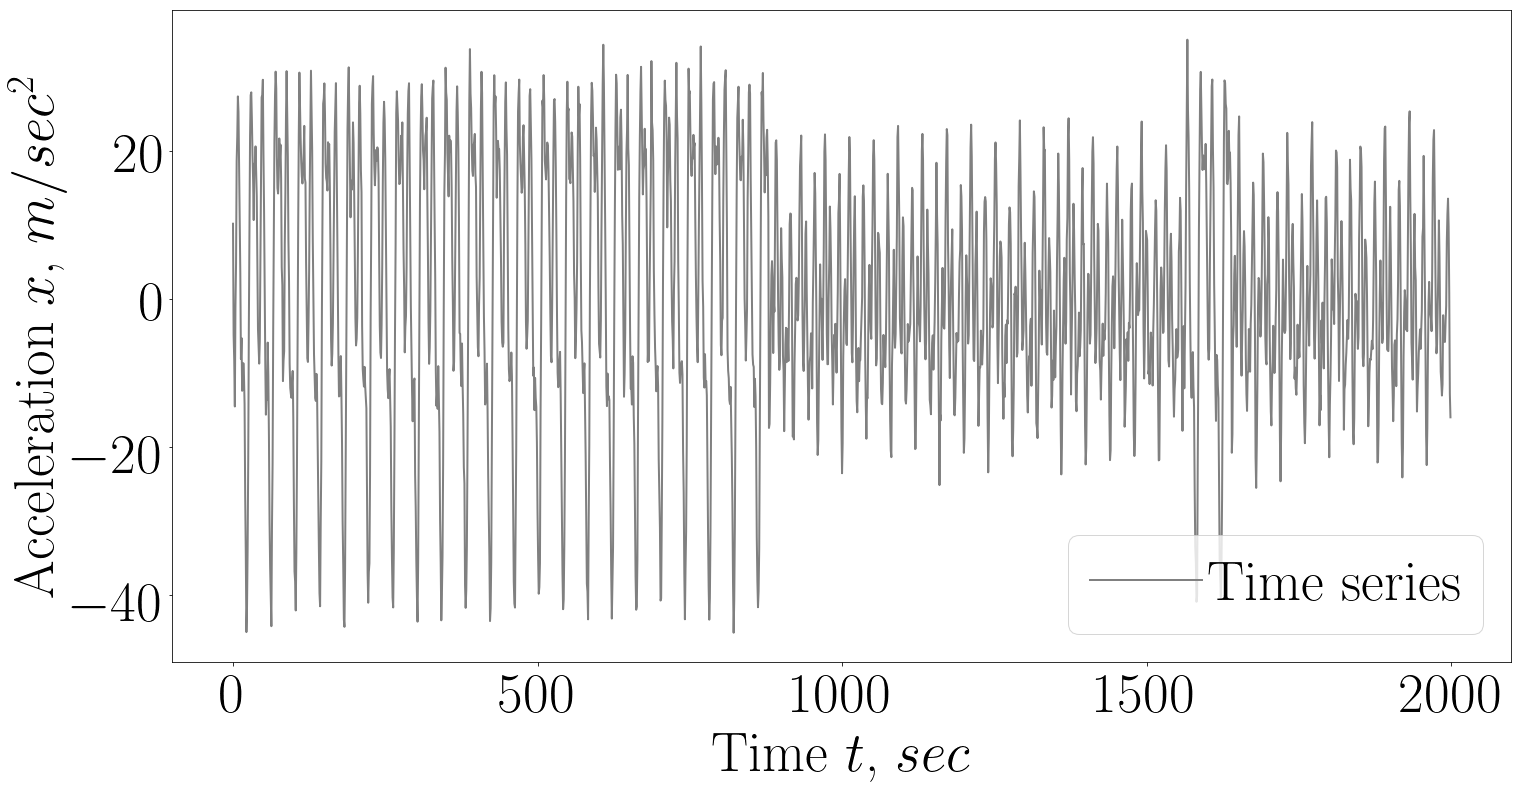
\includegraphics[width=0.5\textwidth]{results/series/2_patern_2_series}\label{fig_synthetic_series_2}}
\subfloat[]
{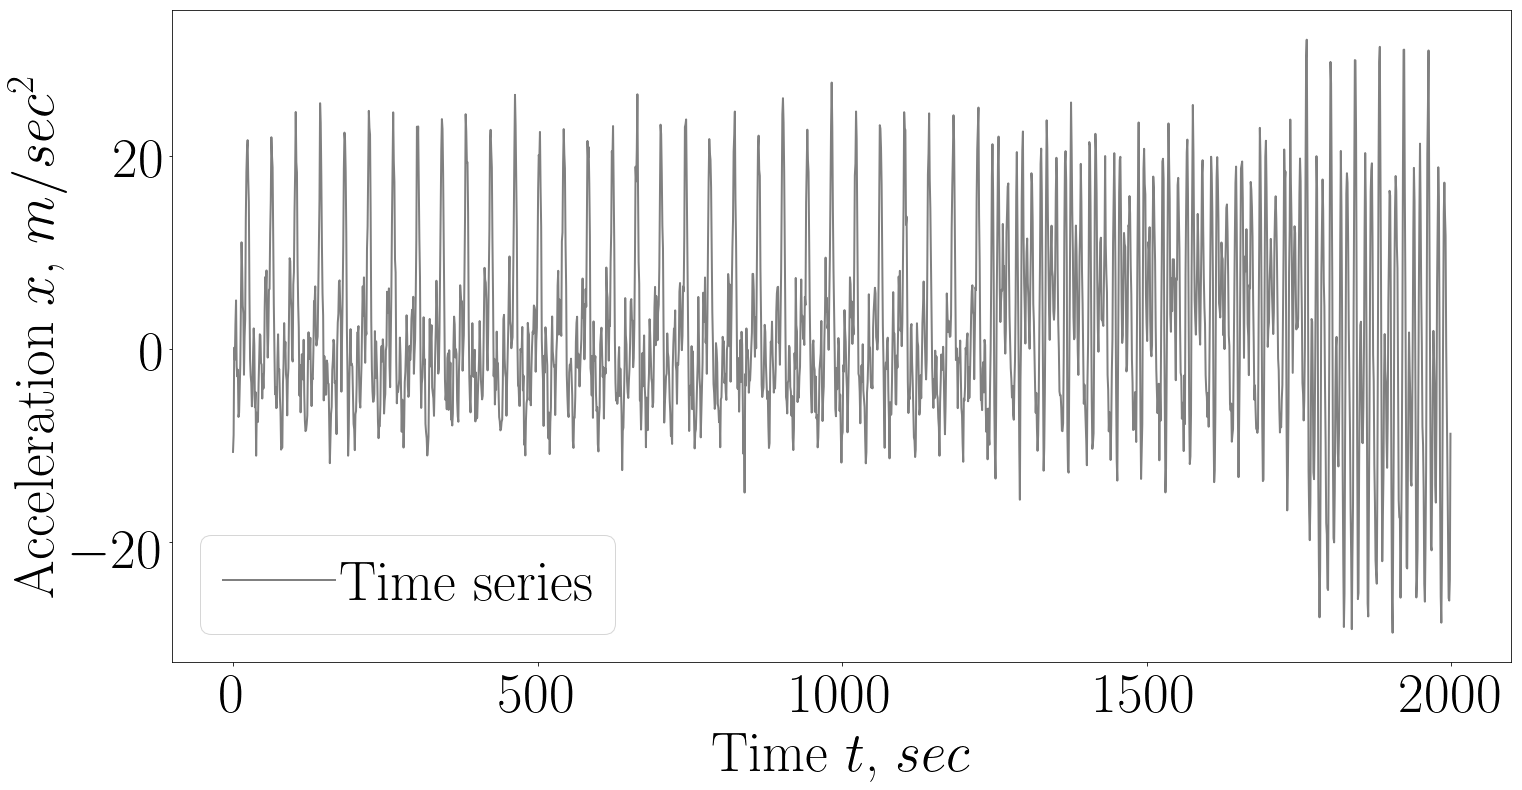
\includegraphics[width=0.5\textwidth]{results/series/3_patern_2_series}\label{fig_synthetic_series_3}}\\
\caption{Пример синтетически построенных временных рядов: a) для временного ряда Synthetic 1; b) для временного ряда Synthetic 2}
\label{fig_synthetic_series}
\end{figure}

\begin{figure}[h!t]\center
\subfloat[]
{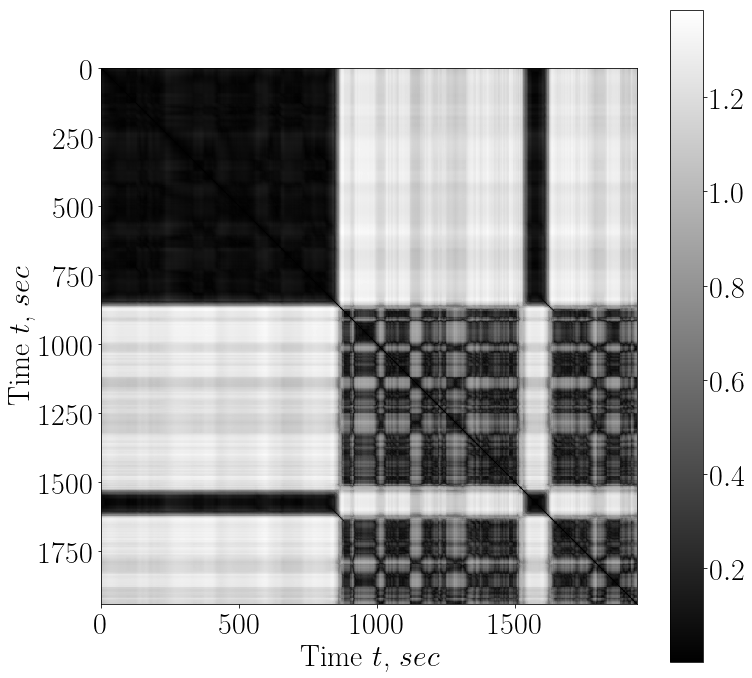
\includegraphics[width=0.5\textwidth]{results/series/2_patern_2_full}}
\subfloat[]
{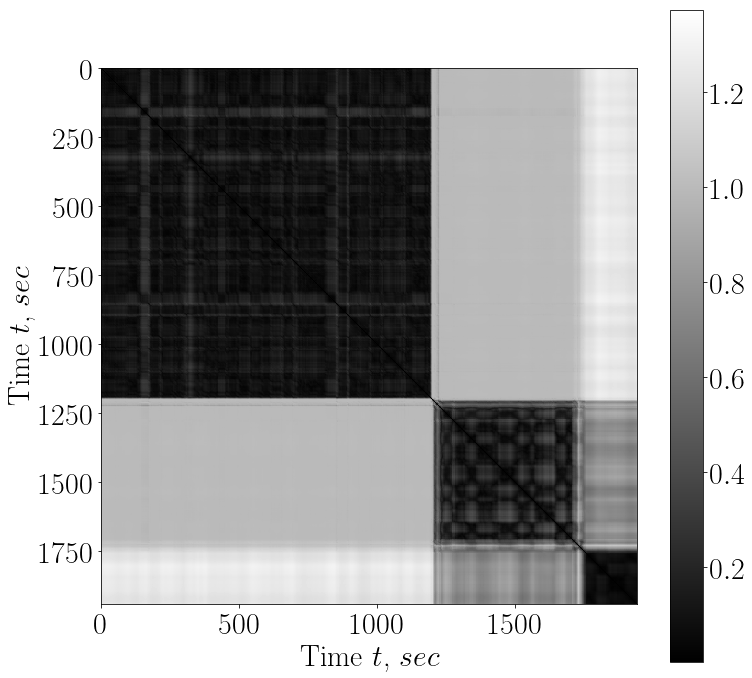
\includegraphics[width=0.5\textwidth]{results/series/3_patern_2_full}}\\
\caption{Матрица попарных расстояний~$\textbf{M}$ между точками временного ряда: a) для временного ряда Synthetic 1; b) для временного ряда Synthetic 2}
\label{fig_synthetic_distance}
\end{figure}

\begin{figure}[h!t]\center
\subfloat[]
{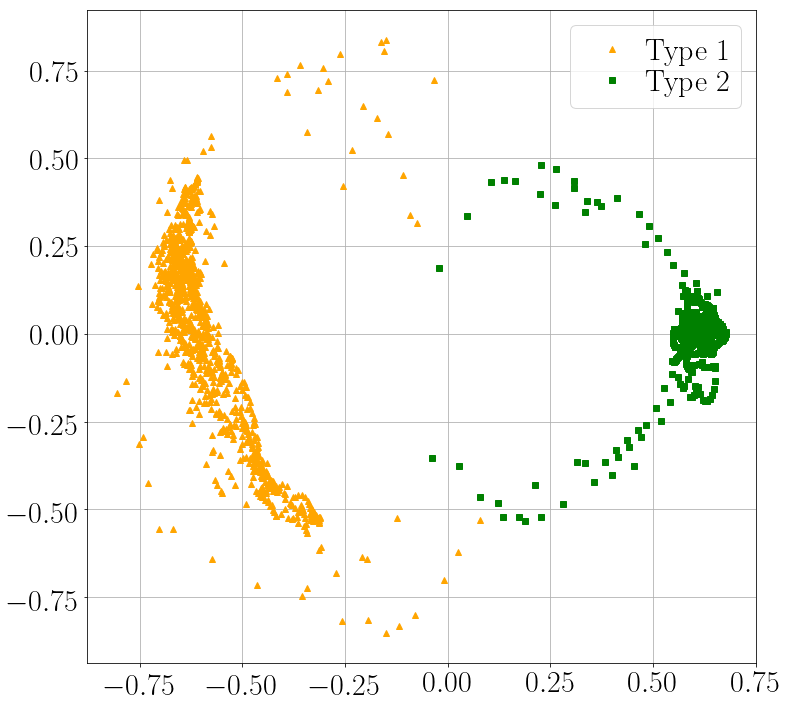
\includegraphics[width=0.5\textwidth]{results/series/2_patern_2_2D_vector}}
\subfloat[]
{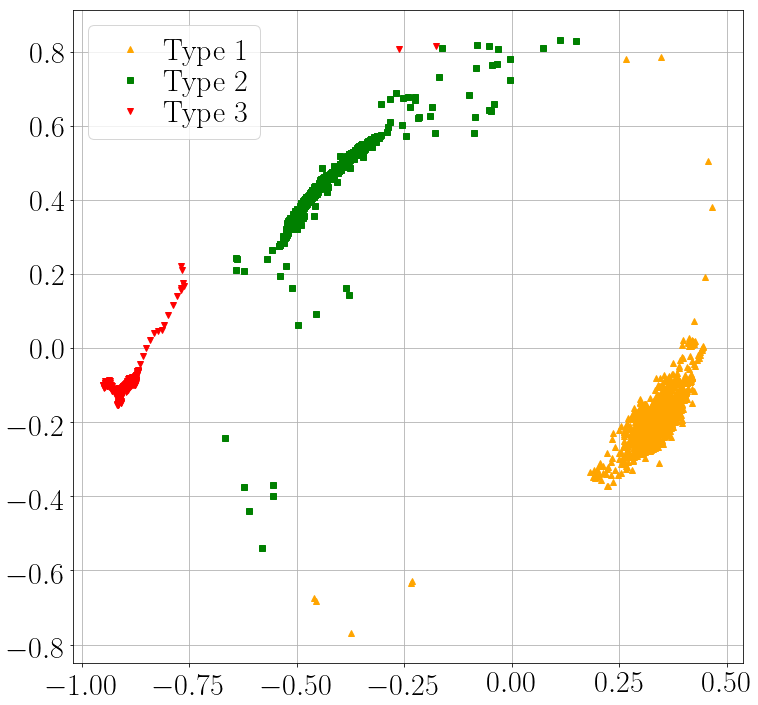
\includegraphics[width=0.5\textwidth]{results/series/3_patern_2_2D_vector}}\\
\caption{Проекция точек временного ряда на плоскость при помощи матрицы попарных расстояний~$\textbf{M}$: a) для временного ряда Synthetic 1; b) для временного ряда Synthetic 2}
\label{fig_synthetic_2D}
\end{figure}

\begin{figure}[h!t]\center
\subfloat[]
{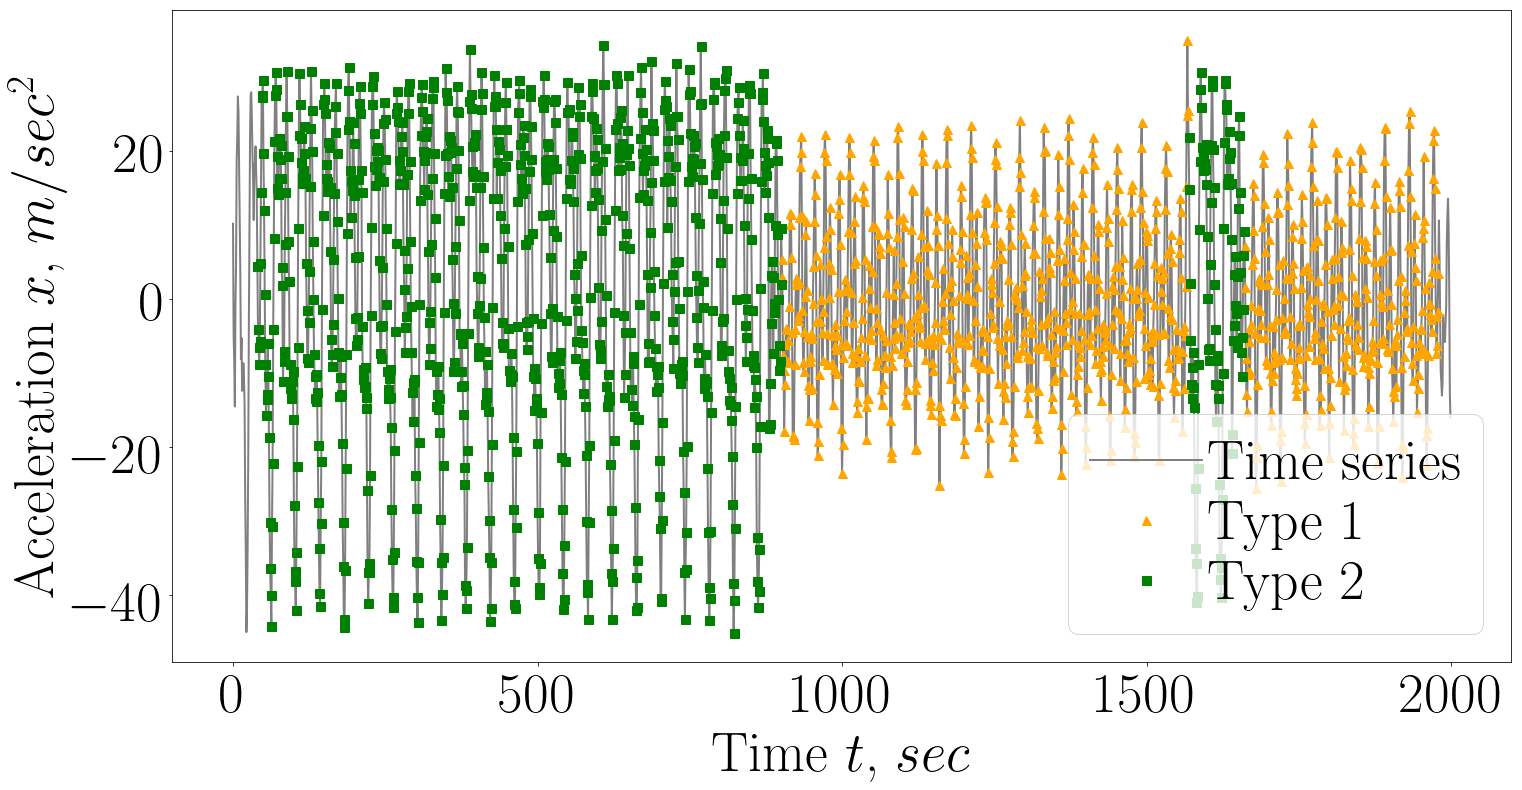
\includegraphics[width=0.5\textwidth]{results/series/2_patern_2_claster_vector}}
\subfloat[]
{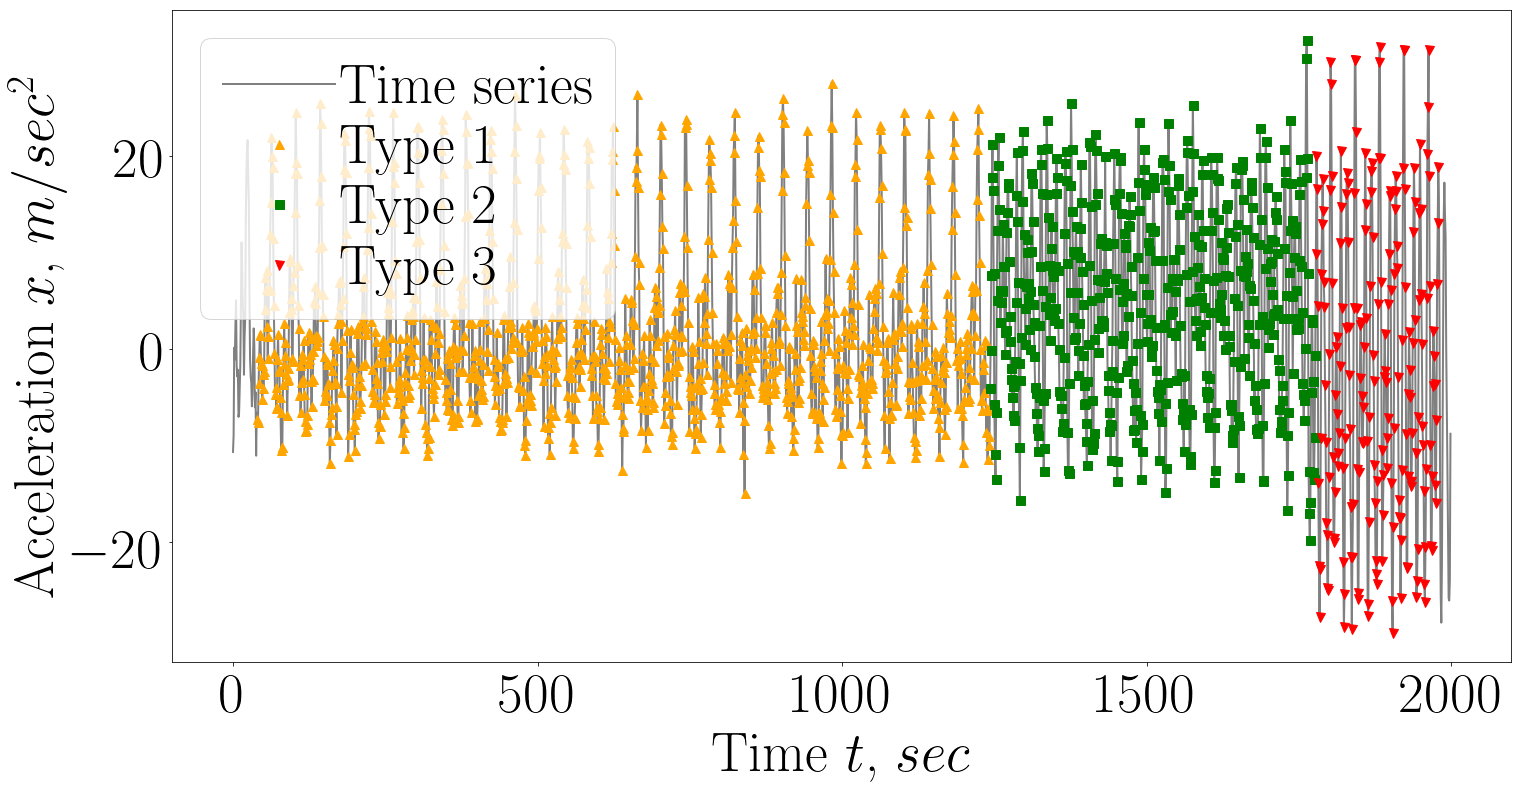
\includegraphics[width=0.5\textwidth]{results/series/3_patern_2_claster_vector}}\\
\caption{Кластеризация точек временного ряда: a) для временного ряда Synthetic 1; b) для временного ряда Synthetic 2}
\label{fig_synthetic_claster}
\end{figure}


На рис. \ref{fig_synthetic_series} приведен пример синтетических временных рядов. 
На рис. \ref{fig_synthetic_series_2} показан пример ряда в котором число различных сегментов~$K = 2$, а длина каждого сегмента~$T = 20$. 
На рис. \ref{fig_synthetic_series_3} показан пример ряда в котором число различных сегментов~$K = 3$, а длина каждого сегмента~$T = 20$. 

Рис. \ref{fig_synthetic_distance} иллюстрирует матрицы попарных расстояний~$\textbf{M}$ между всеми парами точек~$t$ временного ряда, которые построены при помощи (\ref{eq:cl:9}). 
Используя матрицу попарных расстояний и метод многомерного шкалирования~\cite{Borg2005} визуализируем точки временного ряда на плоскости. 
На рис. \ref{fig_synthetic_2D} показана визуализация точек на плоскости и выполнена их кластеризация при помощи метода иерархической кластеризации. 
Иллюстрация кластеров точек временного ряда продемонстрирована на рис. \ref{fig_synthetic_claster}.

\begin{figure}[h!t]\center
\subfloat[]
{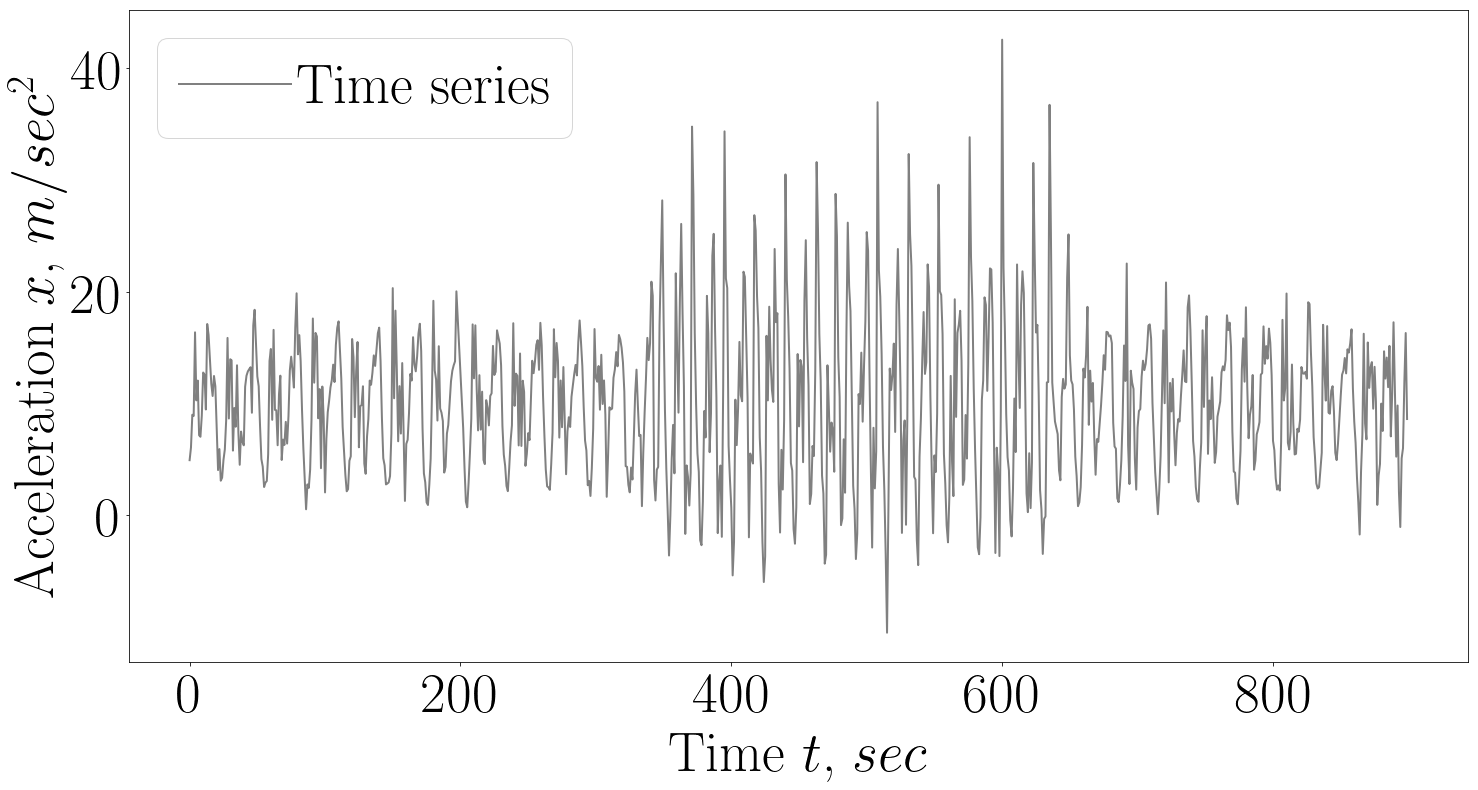
\includegraphics[width=0.5\textwidth]{results/series/real_1_series}}
\subfloat[]
{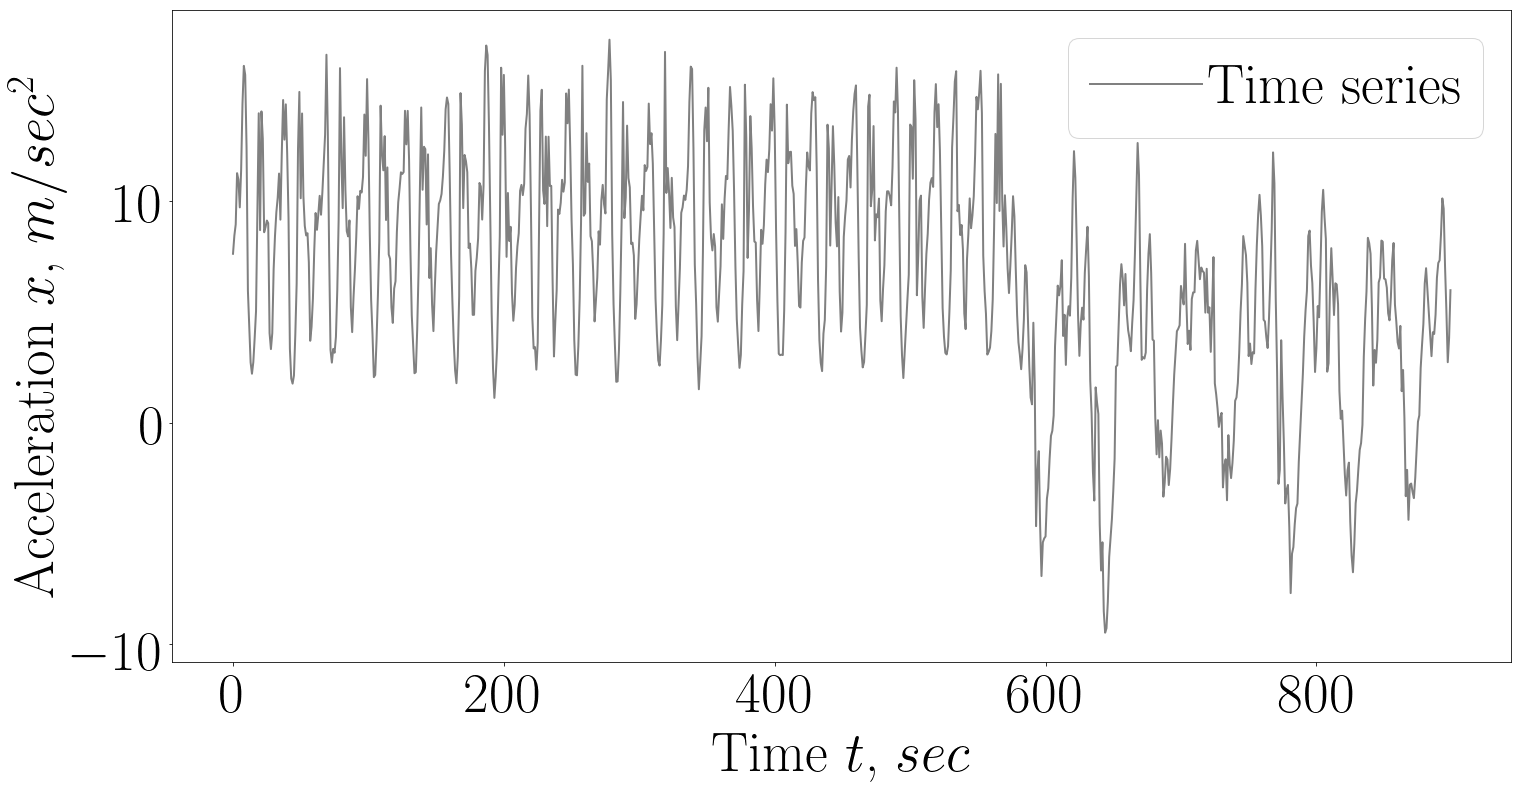
\includegraphics[width=0.5\textwidth]{results/series/real_2_series}}\\
\caption{Пример синтетически построенных временных рядов: a) для временного ряда Physical Motion 1; b) для временного ряда Physical Motion 2}
\label{fig_real_series}
\end{figure}

\begin{figure}[h!t]\center
\subfloat[]
{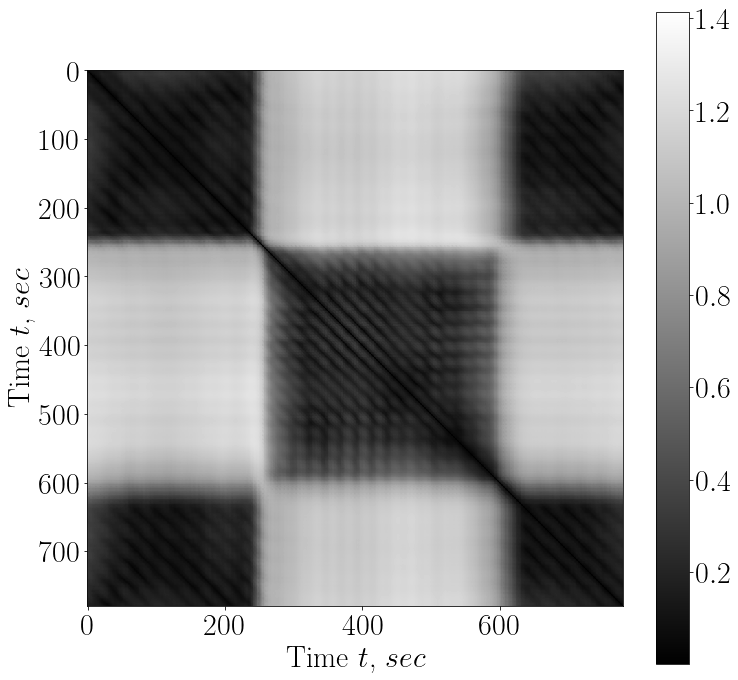
\includegraphics[width=0.5\textwidth]{results/series/real_1_full}}
\subfloat[]
{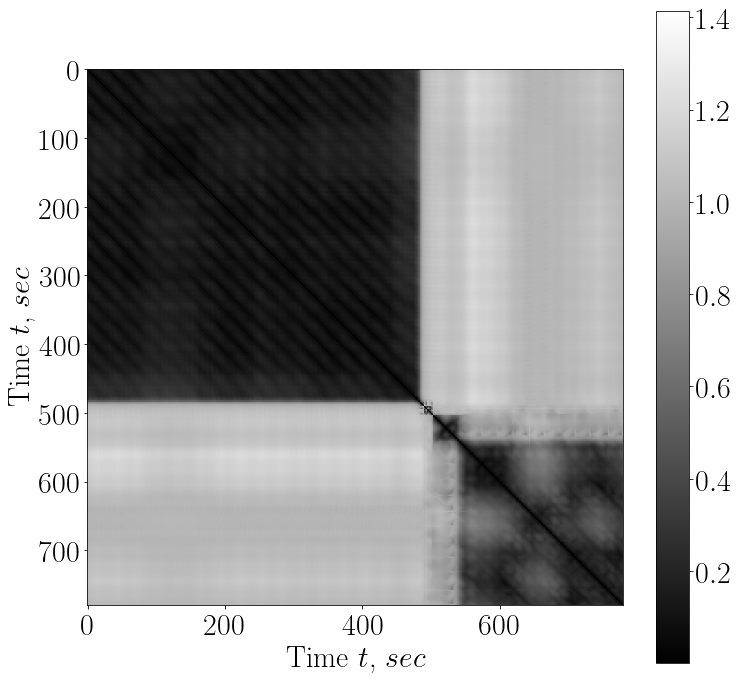
\includegraphics[width=0.5\textwidth]{results/series/real_2_full}}\\
\caption{Матрица попарных расстояний~$\textbf{M}$ между точками временного ряда: a) для временного ряда Physical Motion 1; b) для временного ряда Physical Motion 2}
\label{fig_real_distance}
\end{figure}

\begin{figure}[h!t]\center
\subfloat[]
{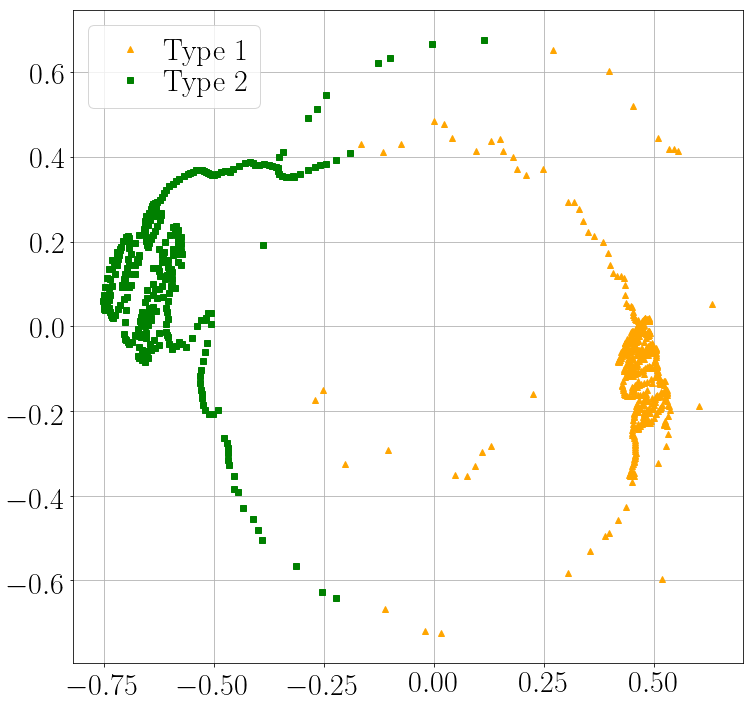
\includegraphics[width=0.5\textwidth]{results/series/real_1_2D_vector}}
\subfloat[]
{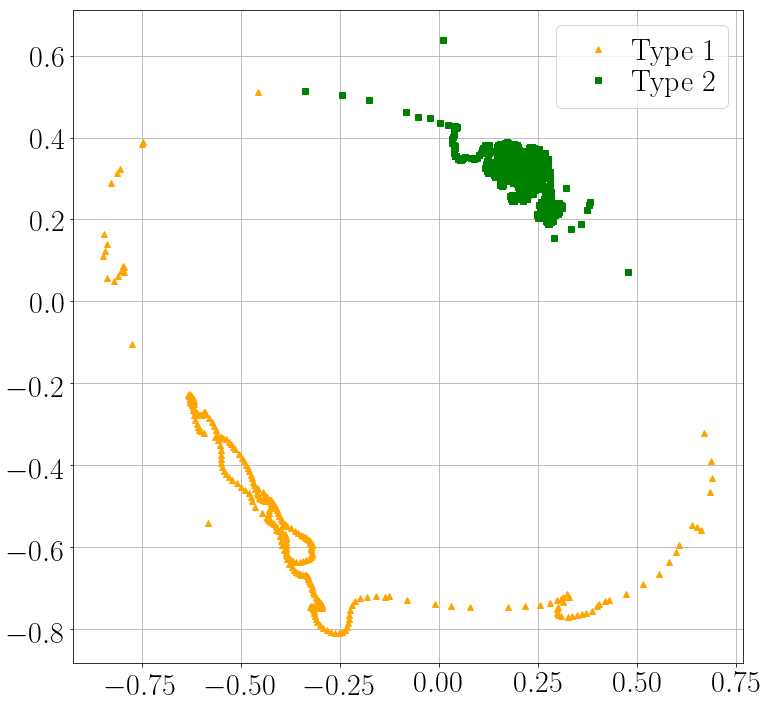
\includegraphics[width=0.5\textwidth]{results/series/real_2_2D_vector}}\\
\caption{Проекция точек временного на плоскость при помощи матрицы попарных расстояний~$\textbf{M}$: a) для временного ряда Physical Motion 1; b) для временного ряда Physical Motion 2}
\label{fig_real_2D}
\end{figure}

\begin{figure}[h!t]\center
\subfloat[]
{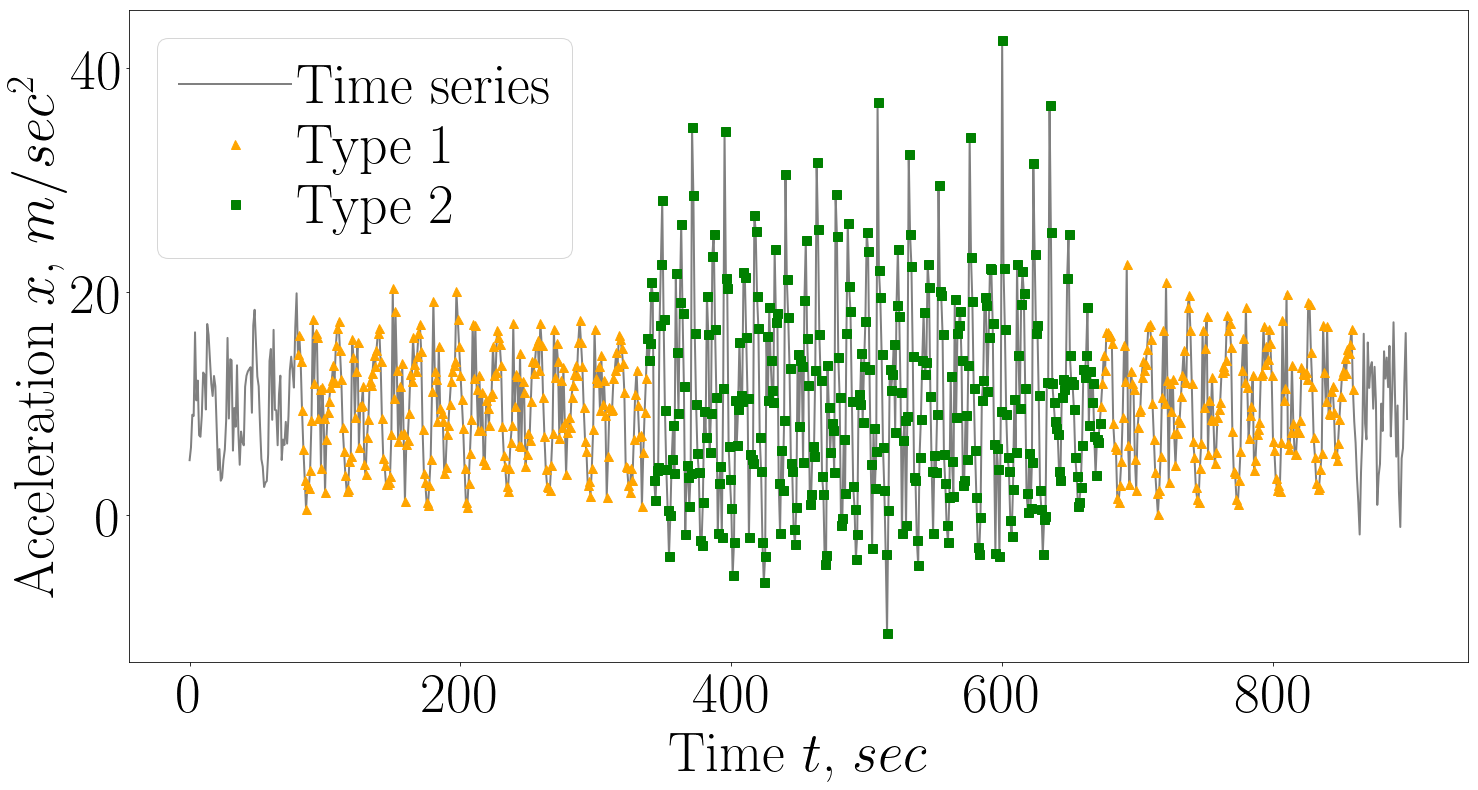
\includegraphics[width=0.5\textwidth]{results/series/real_1_claster_vector}}
\subfloat[]
{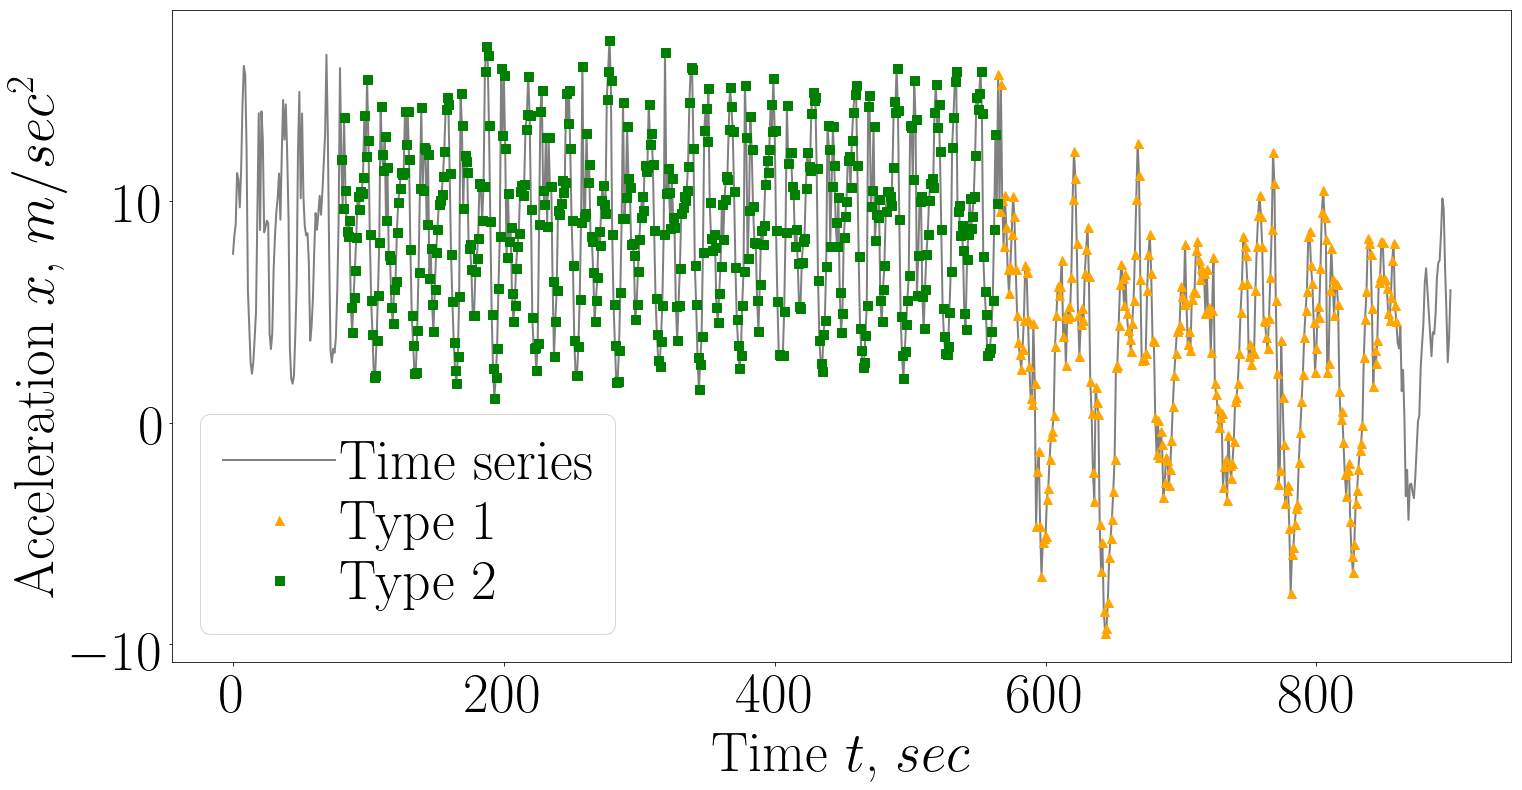
\includegraphics[width=0.5\textwidth]{results/series/real_2_claster_vector}}\\
\caption{Кластеризация точек временного ряда: 
a) для временного ряда Physical Motion 1; b) для временного ряда Physical Motion 2}
\label{fig_real_claster}
\end{figure}

На рис. \ref{fig_real_series} приведен пример реальных временных рядов полученных при помощи взятия одной из координат мобильного акселерометра. 

Рис. \ref{fig_real_distance} иллюстрирует матрицы попарных расстояний~$\textbf{M}$ между всеми парами точек~$t$ временного ряда, которые построены при помощи (\ref{eq:cl:9}). 
Используя матрицу попарных расстояний и метод многомерного шкалирования~\cite{Borg2005} визуализируем точки временного ряда на плоскости. 
На рис. \ref{fig_real_2D} показана визуализация точек на плоскости и выполнена их кластеризация при помощи метода иерархической кластеризации. 
Иллюстрация кластеров точек временного ряда продемонстрирована на рис. \ref{fig_real_claster}.

Сегментация временных рядов проводится на синтетических и реальных данных. Для данного эксперимента в качестве синтетического ряда рассматривается ряд построенный из двух синусов с произвольной частотой и амплитудой. Описание временных рядов, которые используются в данном эксперименте представлены в таблице \ref{table:3}.

Сегментация проводится при помощи метода, который представлен в работе~\cite{motrenko2015}. Данный метод применяется для каждого действия внутри временного ряда по отдельности.


\begin{table}[h!t]
\begin{center}
\caption{Описание временных рядов в эксперименте сегментации временных рядов}
\label{table:3}
\begin{tabular}{|c|c|c|c|}
\hline
	Ряд,~$\textbf{x}$ &Длина ряда,~$N$& Число сегментов,~$K$&Длина сегмента,~$T$\\
	\hline
	\multicolumn{1}{|l|}{Simple 1}
	& 1000& 2& 100\\
	\hline
	\multicolumn{1}{|l|}{Physical Motion 2}
	& 900& 2& 40\\
\hline

\end{tabular}
\end{center}
\end{table}

На рис. \ref{fig_simple_segmentation} показан результат сегментации для временного ряда Simple 1. 
Данный алгоритм хорошо выделил начала сегментов. 
Также на рис. \ref{fig_simple_segmentation} показаны проекции фазовых пространств для обеих кластеров на их первые две главные компоненты.

\begin{figure}[h!t]\center
\subfloat[]
{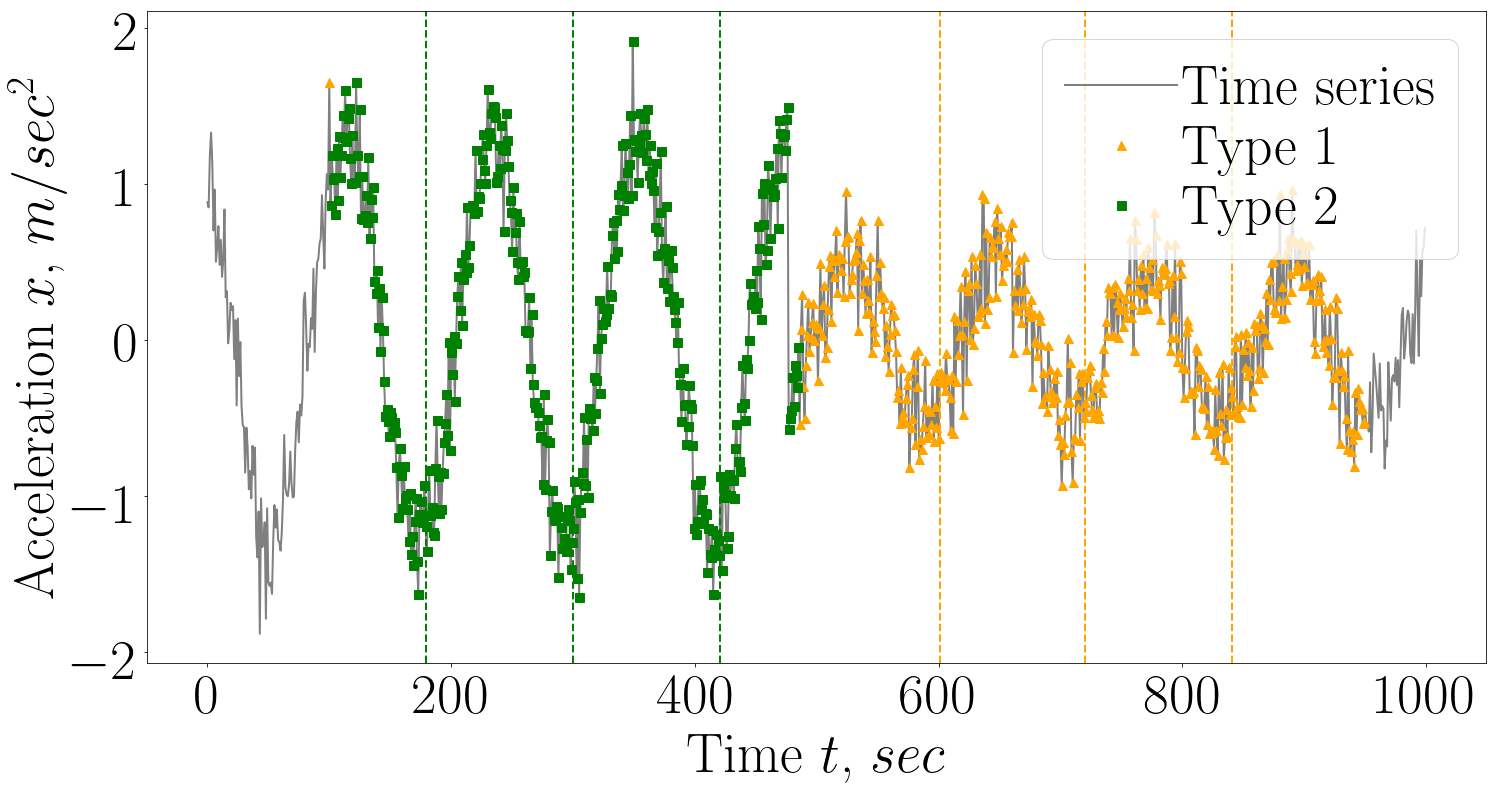
\includegraphics[width=0.5\textwidth]{results/series/simple_1_segmentation_vector}}
\subfloat[]
{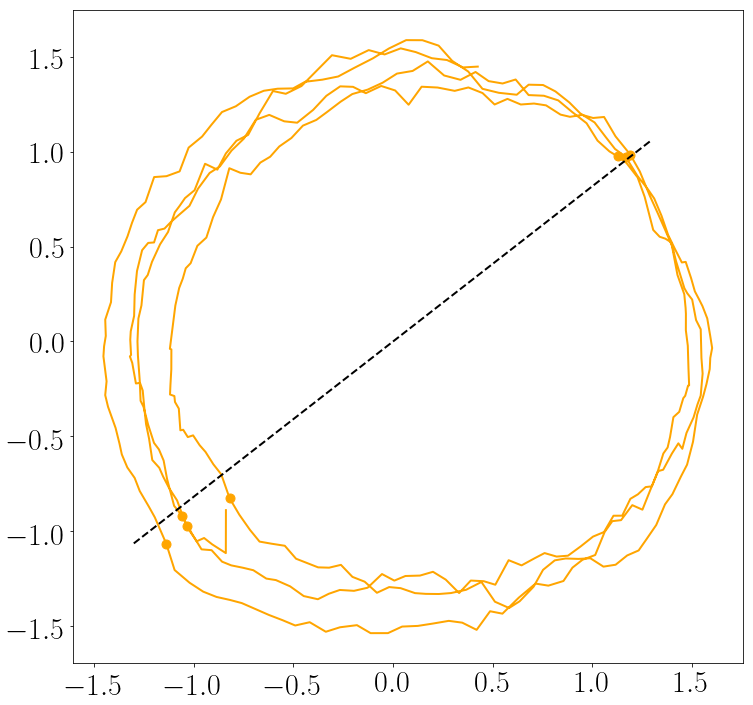
\includegraphics[width=0.25\textwidth]{results/series/simple_1_phase_space0}}
\subfloat[]
{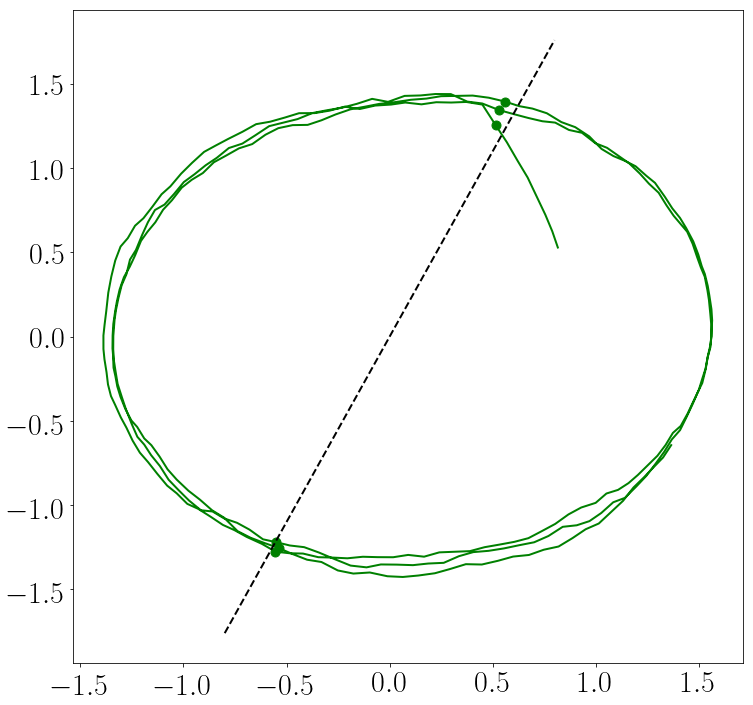
\includegraphics[width=0.25\textwidth]{results/series/simple_1_phase_space1}}\\
\caption{Сегментация точек временного ряда Simple 1: 
a) сегментация временного ряда; b) проекция фазового пространства на первые две главные компоненты для первого кластера; c) проекция фазового пространства на первые две главные компоненты для второго кластера}
\label{fig_simple_segmentation}
\end{figure}

\paragraph{Реальные данные.} На рис. \ref{fig_real_segmentation} показан результат сегментации для временного ряда Physical Motion 2. 
Данный алгоритм хорошо выделил начала сегментов для Type 1 и плохо для Type 2. 
Также на рис. \ref{fig_real_segmentation} показаны проекции фазовых пространств для обеих кластеров на их первые две главные компоненты. 
Видно, что в случае проекции фазового пространства для части ряда, который относится к Type 2 получаем, что фазовая траектория имеет самопересечение внутри одного сегмента, что влечет нахождения ложного начала сегмента.

\begin{figure}[h!t]\center
\subfloat[]
{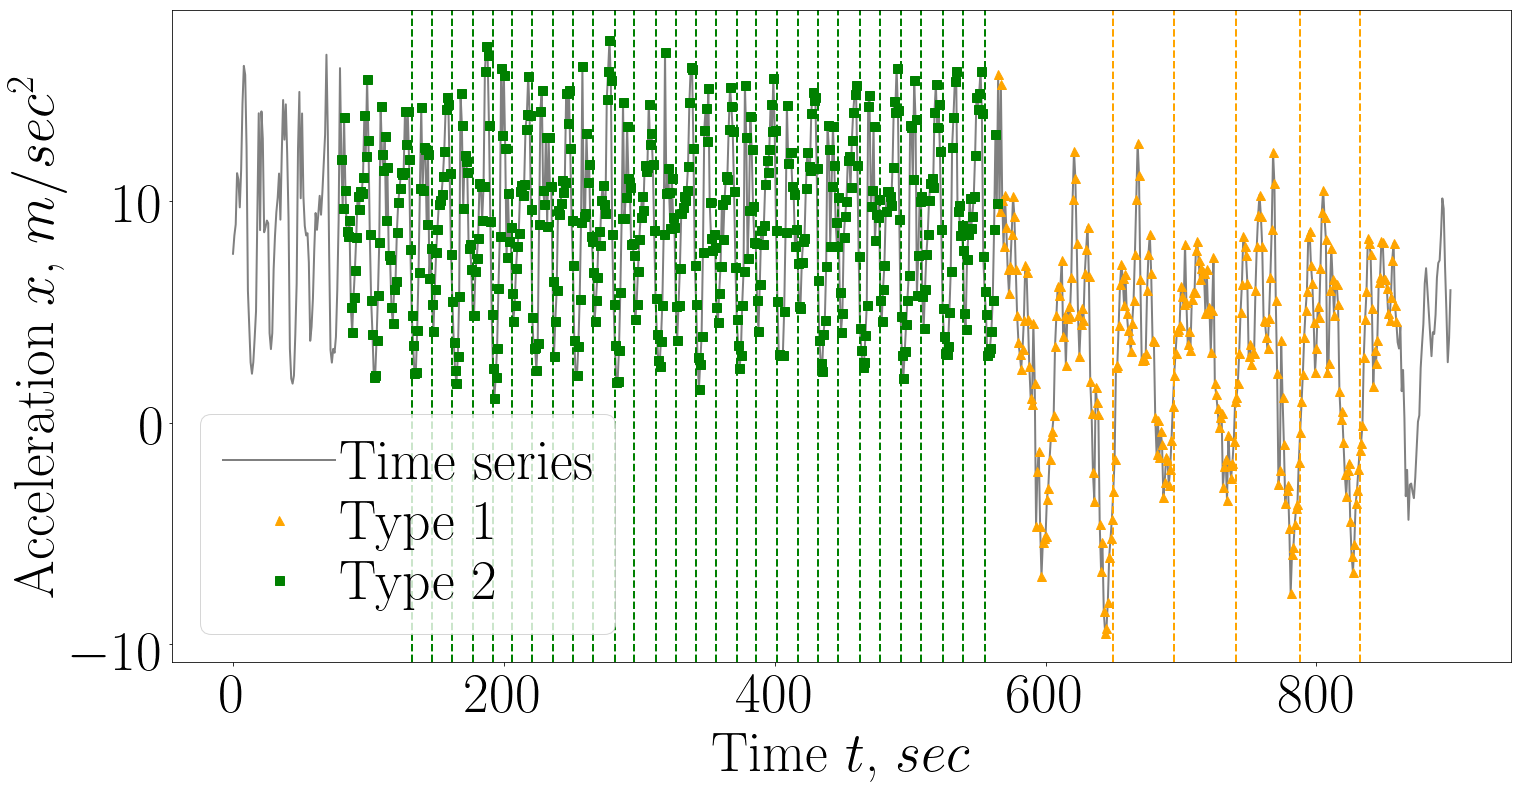
\includegraphics[width=0.5\textwidth]{results/series/real_2_segmentation_vector}}
\subfloat[]
{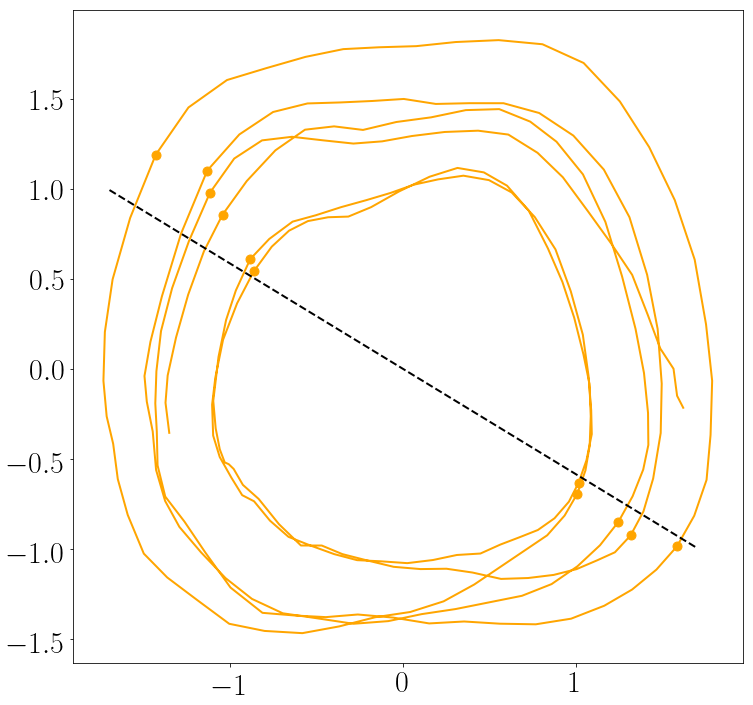
\includegraphics[width=0.25\textwidth]{results/series/real_2_phase_space0}}
\subfloat[]
{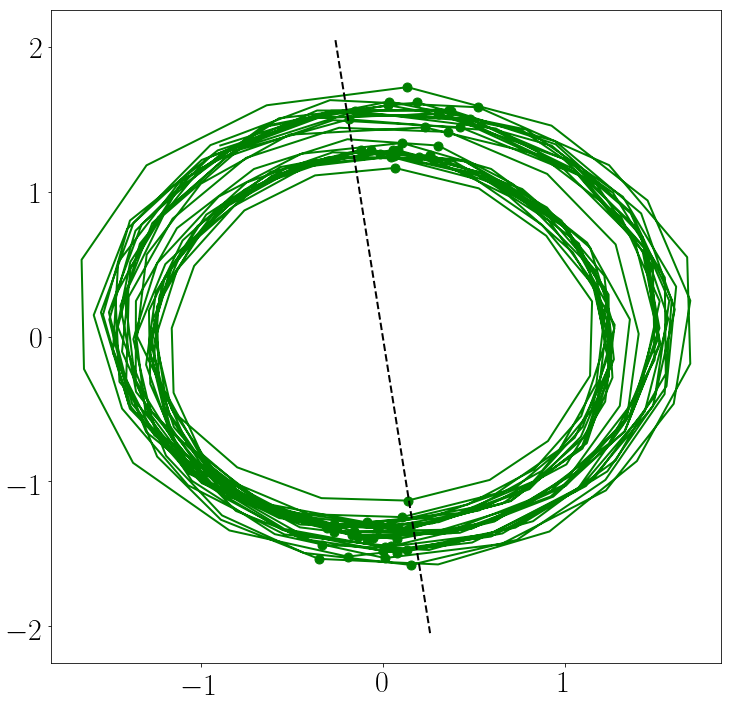
\includegraphics[width=0.25\textwidth]{results/series/real_2_phase_space1}}\\
\caption{Сегментация точек временного ряда Physical Motion 2: 
a) сегментация временного ряда; b) проекция фазового пространства на первые две главные компоненты для первого кластера; c) проекция фазового пространства на первые две главные компоненты для второго кластера}
\label{fig_real_segmentation}
\end{figure}